	\documentclass[10pt]{beamer}
	\usepackage{tikz}
	\usepackage{stmaryrd}
	\usepackage{beamerthemesplit}
	\usepackage{xcolor}
	\usepackage{hyperref}
	% \usepackage[utf8x]{inputenc}
	
	
	\newcommand{\TSync}[0]{\ltimes}
	\newcommand{\TWait}[0]{\rtimes}
	\newcommand{\TTot}[0]{\bowtie}
	
	
	\usetheme{Warsaw}
	% per trasparenza su animazioni di blocchi
	\setbeamercovered{dynamic}
	
	
	
	%\title{Rupos: Process analysis and ProM development}
	\title{Rupos Demo: Process analysis into ProM}
	\author[Bruni, Corradini, Ferrari, Guanciale, \alert{Spagnolo}]{Roberto Bruni \and Andrea Corradini  \and Gianluigi Ferrari\\ 
	Roberto Guanciale  \and \alert{Giorgio Spagnolo}}
	%\author{Andrea Corradini}
	\institute{Dipartimento di Informatica, Pisa}
	\date{RUPOS Demo \\ 22 Marzo 2012}
	
	\begin{document}
	\frame{\titlepage}
	
	\section{Sommario}
	
	%% \begin{frame}
	%% %\frame{
	
	%%   \begin{block}{Il gruppo del Dipartimento di Informatica}
	%%     \begin{itemize}
	%%     \item Roberto Bruni, ricercatore
	%%     \item Andrea Corradini, professore associato [responsabile]
	%%     \item Gianluigi Ferrari, professore associato\\[5mm]
	
	%%     \item Silvia Bertagnini, contrattista [OO6 - Disseminazione]
	%%     \item Roberto Guanciale, borsista [OO2]
	%%     \item Giorgio Spagnolo, borsista  [OO2]\\[5mm]
	
	
	%% \item Giovanni Bussu, tesista
	%% \item Emilio Ferro, tesista [Dicembre 2010]
	%% \item Hind Chfouka, tirocinante
	%% \item Leonardo Venezia, tirocinante
	%% \end{itemize}
	%% \end{block}
	%% \end{frame}
	%}  
	
	%\begin{frame}
	%\begin{block}{Attivit\`{a} previste per l'Obiettivo Operativo 2} 
	%\begin{description}
	%\item[A2.1] Linguaggi e modelli per pattern fondamentali\\
	%\begin{itemize}
	% \item Attivit\`{a} di rassegna sullo stato dell'arte
	%\item Prevede rilascio di documento di rassegna
	%\end{itemize}
	%\item[A2.2] Analisi e verifica dei pattern fondamentali
	%\begin{itemize}
	% \item Attivit\`{a} di ricerca di base e applicata
	%\item Prevede rilascio di documento di ricerca 
	%\end{itemize}
	%\item[A2.3] Middleware prototipale
	%\begin{itemize}
	% \item Attivit\`{a} di sviluppo software
	%\item Prevede rilascio di software e documentazione 
	%\end{itemize}
	%\end{description}
	%\end{block}
	%\end{frame}
	%
	%\section{[A2.1] Linguaggi e modelli per pattern fondamentali}
	%\begin{frame}{[A2.1] Linguaggi e modelli per pattern fondamentali}
	%
	%%Attivit\`{a} di rassegna su formalismi di riferimento per applicazioni SOA
	%%%  la progettazione di applicazioni SOA. 
	%%% differenziando i modelli per la specifica, dai modelli
	%%% semantici. Presentiamo anche una rassegna di mapping tra i modelli
	%%% proposti e dei tool di traduzione tra di essi. Inoltre descriviamo
	%%% separatamente i meccanismi che i vari modelli offrono per modellare il
	%%% concetto di sessione.  
	%
	%\begin{block}<1->{Rassegna su Modelli di Specifica per Applicazioni SOA}
	%\begin{itemize}
	%\item BPMN
	%\item BPEL
	%\item YAWL
	%\end{itemize}
	%\end{block}
	%
	%\begin{block}<2->{Rassegna su Algoritmi e Tool di Traduzione}
	%\begin{itemize}
	%\item BPMN 1.1 to BPEL
	%\item BPMN to YAWL
	%\item BPEL to YAWL
	%\end{itemize}
	%\end{block}
	%
	%\begin{block}<3->{Rassegna su Modelli Formali: Reti di Petri}
	%\end{block}
	%
	%\begin{block}<4->{Rassegna su Supporto per Sessioni con Correlation Set (in BPEL e BPMN)}
	%\end{block}
	%\end{frame}
	
	\section{Analisi e verifica dei pattern fondamentali}
	\subsection{Sommario}
	\begin{frame}{ Analisi e verifica dei pattern fondamentali}
	  \begin{block}{Obiettivo}
	\begin{itemize}
	  \item Integrare in RUPOS strumenti di analisi a runtime di processi
	  \item  Analisi basata sul confronto di logs con un modello del processo
	\end{itemize}
	\end{block}
	
	  \begin{block}<2->{Strategia}
	    \begin{itemize}
	    \item Adottare e raffinare  metodi formali disponibili (Reti di Petri)
	    \item Integrare ed estendere infrastrutture software esistenti (ProM)
	    \item Work-flow metodologico:
	      \begin{enumerate}
	      \item I processi di business sono modellati con diagrammi BPMN
	      \item I diagrammi BPMN vengono trasformati in Reti di Petri
	      \item I logs di Istanze di Processi vengono analizzati con tecniche disponibili per Reti di Petri, oppurtunamente raffinate
	      \item I risultati dell'analisi vengono proiettati sul modello BPMN iniziale
	      \end{enumerate}
	    \end{itemize}
	
	  \end{block}
	\end{frame}
	
	\section{Framework di analisi}
	\begin{frame}
	\frametitle{Framework di analisi}
%	Tecnologie impiegate
%	\begin{itemize}
%	\item Process mining: ProM 6
%	\item Data mining: Weka
%	\item Linguaggio: Java
%	\end{itemize}
	\begin{figure}
	\centering 
	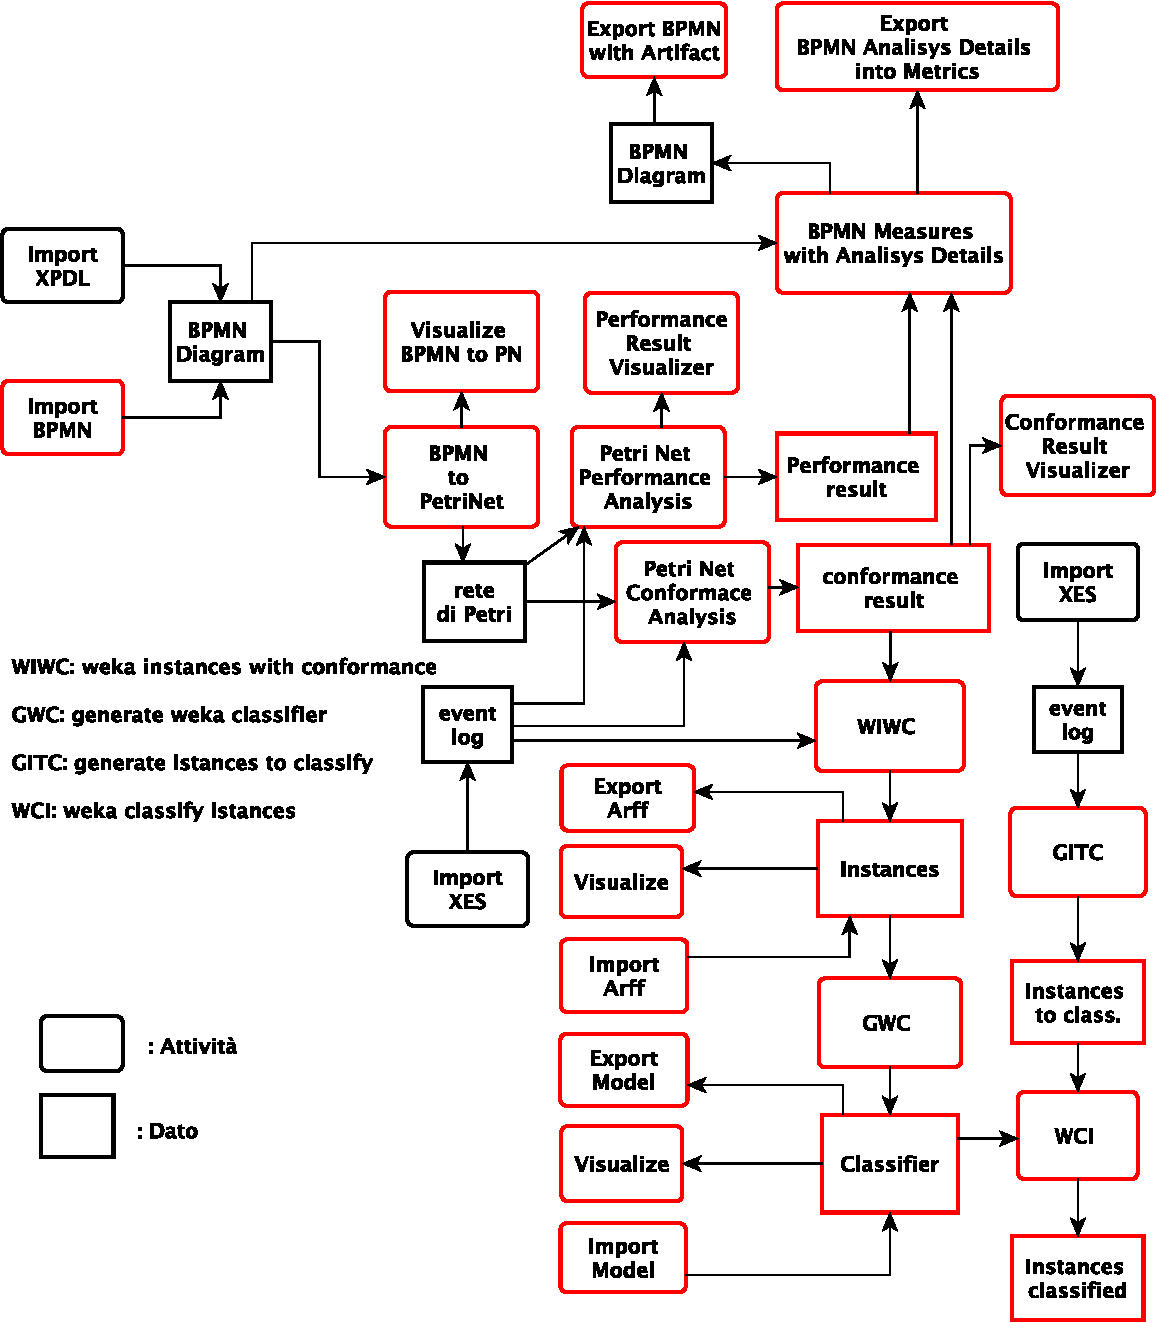
\includegraphics[scale=0.60]{./fig/PromPlugin_pres}
	%\caption{\small{Flusso operativo}}
	\end{figure}
	\end{frame}
	
	% VECCHIO PEZZO DElL'ARCHITETTURA
	% \section{The The Process Monitoring platform}
	% \subsection{Engineering efforts}
	
	%\frame{
  \begin{block}{Overall architecture}
    
    \begin{itemize}
    \item \alert{ProM} an existing process analysis framework
    \item \alert{OpenSPCoop} the most adopted  open source SPCoop implementation
    \end{itemize}

  \end{block}
  \begin{center}
    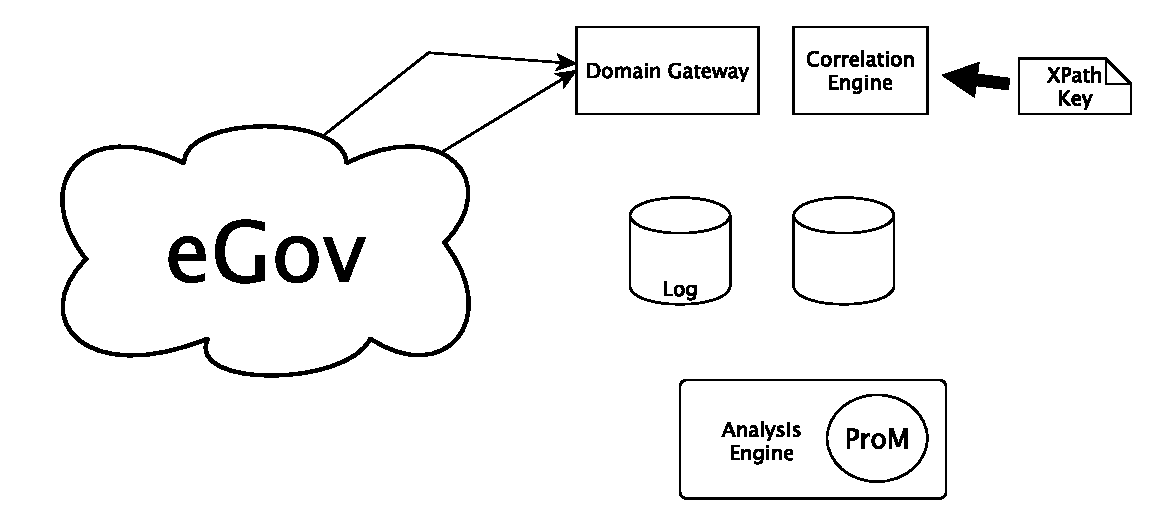
\includegraphics[scale=0.30]{./fig/Platform01}
  \end{center}

}

\frame{
  \begin{block}{Overall architecture}
    
    \begin{itemize}
    \item \alert{ProM} an existing process analysis framework
    \item \alert{OpenSPCoop} the most adopted  open source SPCoop implementation
    \end{itemize}

  \end{block}
  
  \begin{center}
    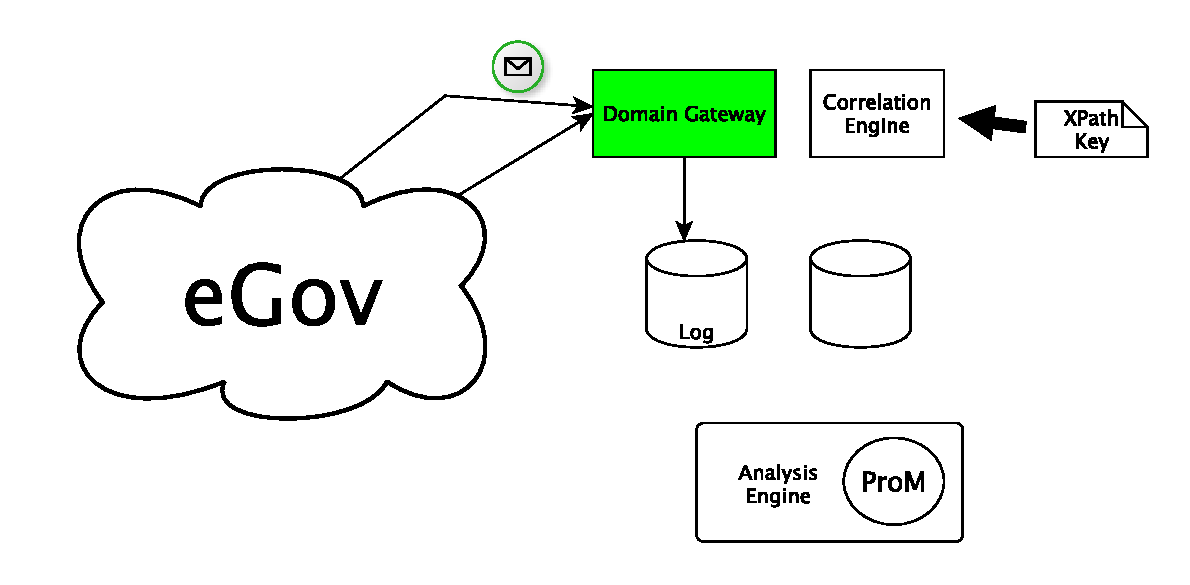
\includegraphics[scale=0.30]{./fig/Platform02}
  \end{center}

  \begin{itemize}
    \item eGov envelopes intercepted by Domain Gateway
    \item Domain Gateway stores message key information into the Log
      database
    %\item Domain Gateway performance are not affected by the analysis
    % \item <2-> Correlation engine groups SOAP request/response
    %   \begin{itemize}
    %     \item exploiting correlation sets (\alert{XPath})
    %     \item annotates process instances into log requests
    %     \item is externally triggered (e.g. cron/trigger)
    %   \end{itemize}
    % \item <3-> Analysis engine evaluates process metrics
    %   \begin{itemize}
    %     \item process definition stored in an external database (\alert{BPMN})
    %     \item process metrics stored into the log database
    %     \item is externally triggered (e.g. cron/trigger)
    %     \item fuffa su ProM
    %   \end{itemize}
  \end{itemize}
}

\frame{
  \begin{block}{Overall architecture}
    
    \begin{itemize}
    \item \alert{ProM} an existing process analysis framework
    \item \alert{OpenSPCoop} the most adopted  open source SPCoop implementation
    \end{itemize}

  \end{block}
  
  \begin{center}
    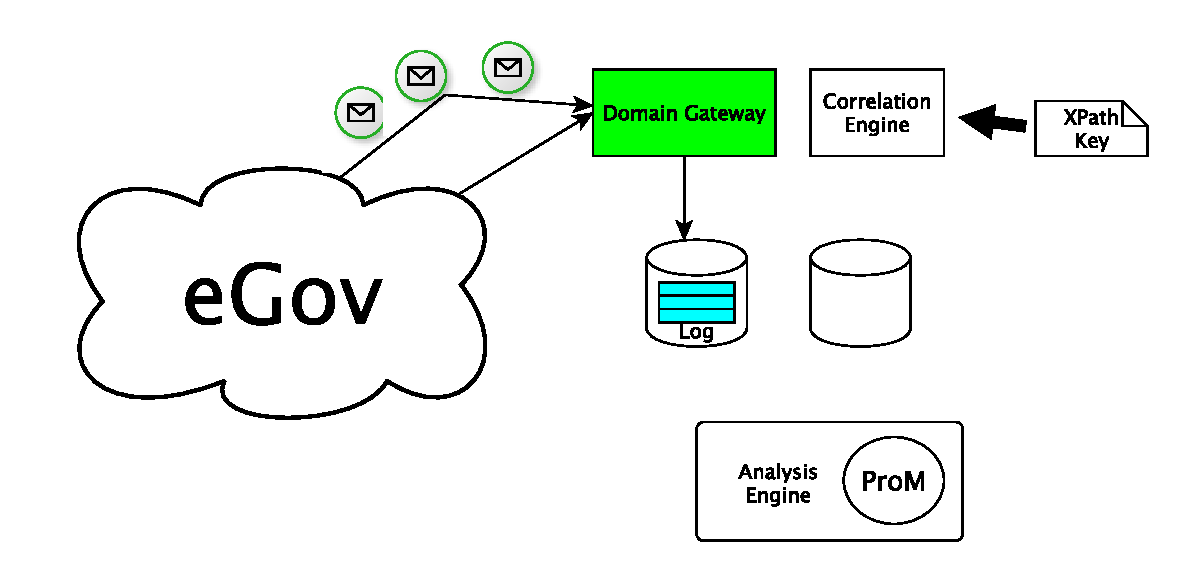
\includegraphics[scale=0.30]{./fig/Platform03}
  \end{center}

  \begin{itemize}
    \item eGov envelopes intercepted by Domain Gateway
    \item Domain Gateway retrieves messages parts storing into the Log
      database
    %\item Domain Gateway performance are not affected by the analysis
    % \item <2-> Correlation engine groups SOAP request/response
    %   \begin{itemize}
    %     \item exploiting correlation sets (\alert{XPath})
    %     \item annotates process instances into log requests
    %     \item is externally triggered (e.g. cron/trigger)
    %   \end{itemize}
    % \item <3-> Analysis engine evaluates process metrics
    %   \begin{itemize}
    %     \item process definition stored in an external database (\alert{BPMN})
    %     \item process metrics stored into the log database
    %     \item is externally triggered (e.g. cron/trigger)
    %     \item fuffa su ProM
    %   \end{itemize}
  \end{itemize}
}

\frame{
  \begin{block}{Overall architecture}
    
    \begin{itemize}
    \item \alert{ProM} an existing process analysis framework
    \item \alert{OpenSPCoop} the most adopted  open source SPCoop implementation
    \end{itemize}

  \end{block}
  
  \begin{center}
    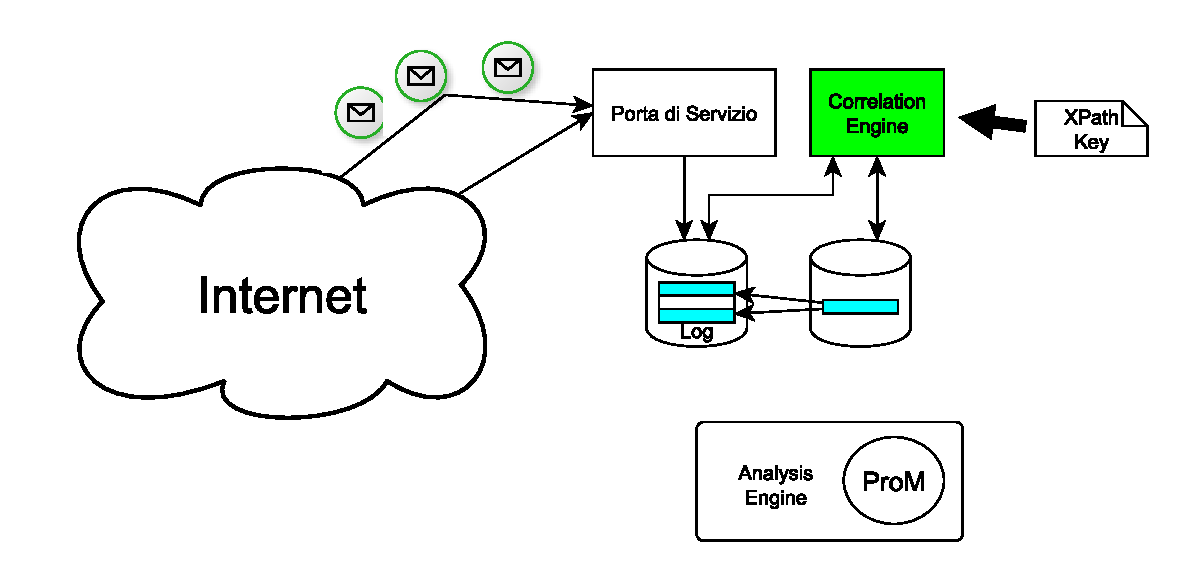
\includegraphics[scale=0.30]{./fig/Platform04}
  \end{center}

  \begin{itemize}
    \item Correlation engine groups SOAP request/response
       exploiting correlation sets (\alert{XPath})
     \item Service externally invoked (e.g. cron/trigger)
    % \item <3-> Analysis engine evaluates process metrics
    %   \begin{itemize}
    %     \item process definition stored in an external database (\alert{BPMN})
    %     \item process metrics stored into the log database
    %     \item is externally triggered (e.g. cron/trigger)
    %     \item fuffa su ProM
    %   \end{itemize}
  \end{itemize}
}

\frame{
  \begin{block}{Overall architecture}
    
    \begin{itemize}
    \item \alert{ProM} an existing process analysis framework
    \item \alert{OpenSPCoop} the most adopted  open source SPCoop implementation
    \end{itemize}

  \end{block}
  
  \begin{center}
    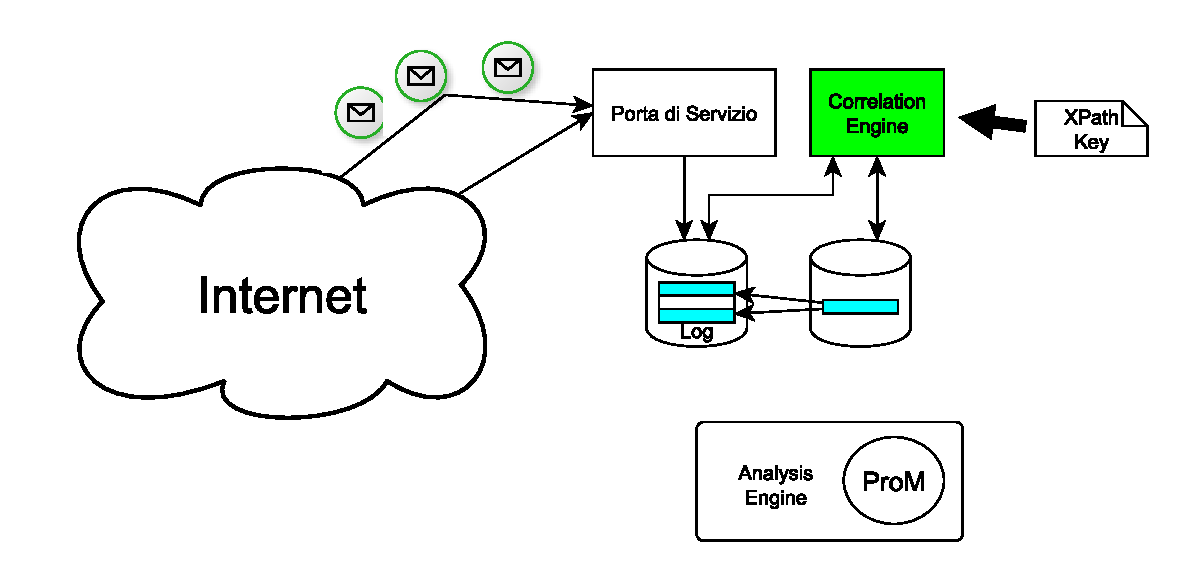
\includegraphics[scale=0.30]{./fig/Platform04}
  \end{center}

  \begin{itemize}
    \item Analysis engine evaluates process metrics
    \item Service externally invoked (e.g. cron/trigger)
    \item implements a context to integrate ProM into JBoss AS
  \end{itemize}
}

%%% Local Variables: 
%%% mode: latex
%%% TeX-master: "main"
%%% End: 

	
	\section{BPMN modeling}
	\begin{frame}{Esempio di processo BPMN}
	  
	  \begin{center}
	    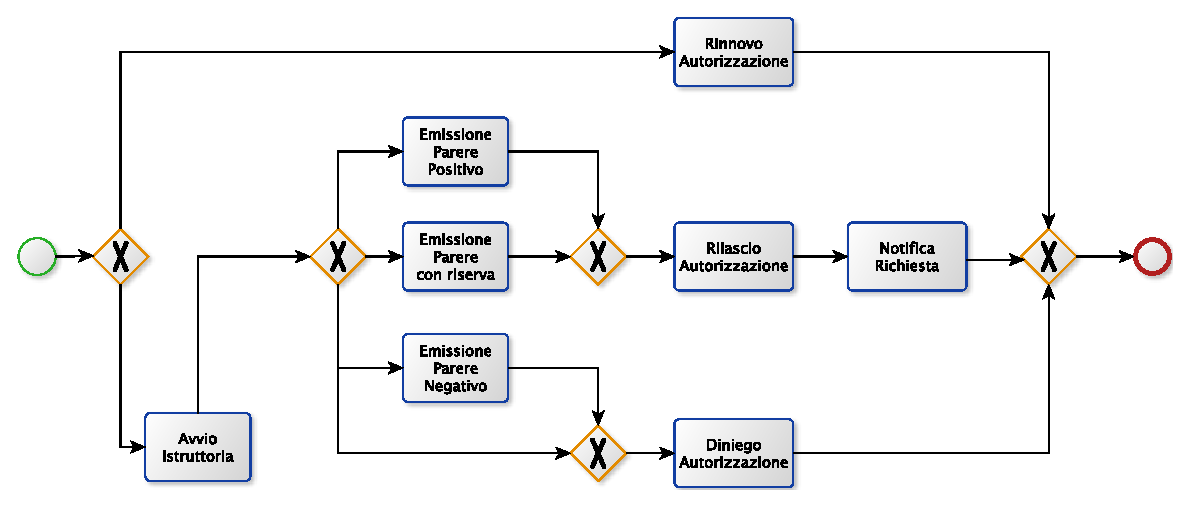
\includegraphics[scale=0.55]{./fig/BPMN}
	  \end{center}
	\end{frame}
	
	\subsection{Traduzione BPMN -- Rete di Petri}
	\begin{frame}{Esempio di processo BPMN e di traduzione in Rete di Petri}
	  
	  \begin{center}
	    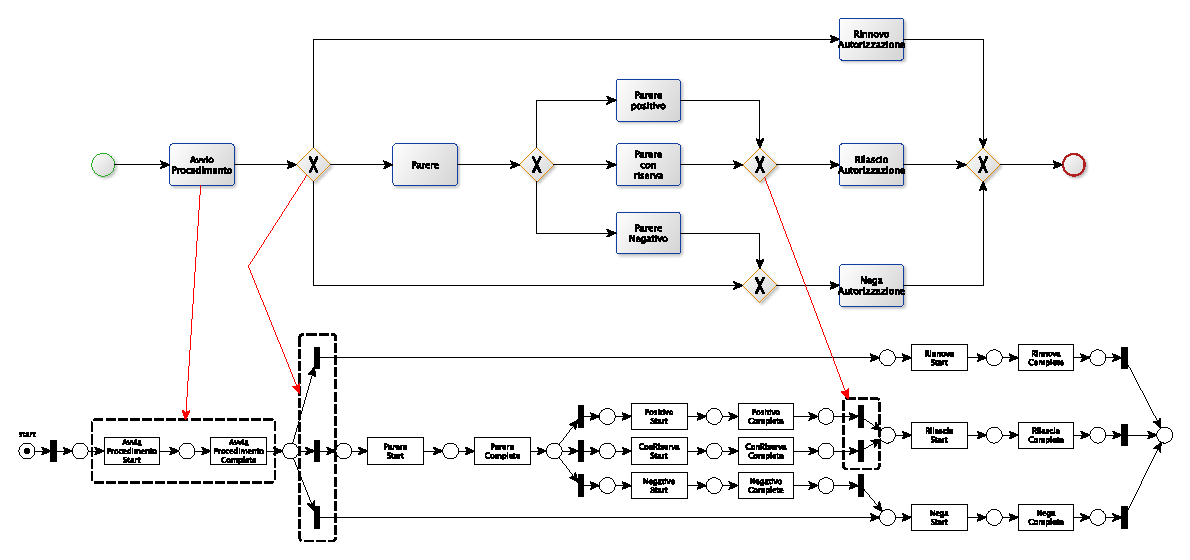
\includegraphics[scale=0.55]{./fig/BPMNandPN}
	  \end{center}
	\end{frame}
	
	
	
	
	%\begin{frame}{Animazione Conformance}
% 
%  
%  \begin{center}
%    
%    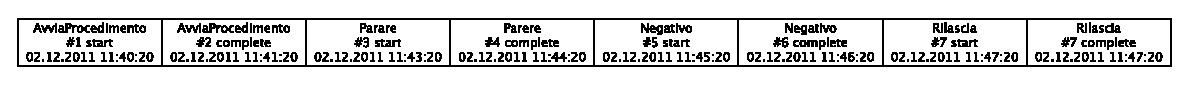
\includegraphics[scale=0.7]{./fig/animazioneconf/log}\\[10pt]
%	    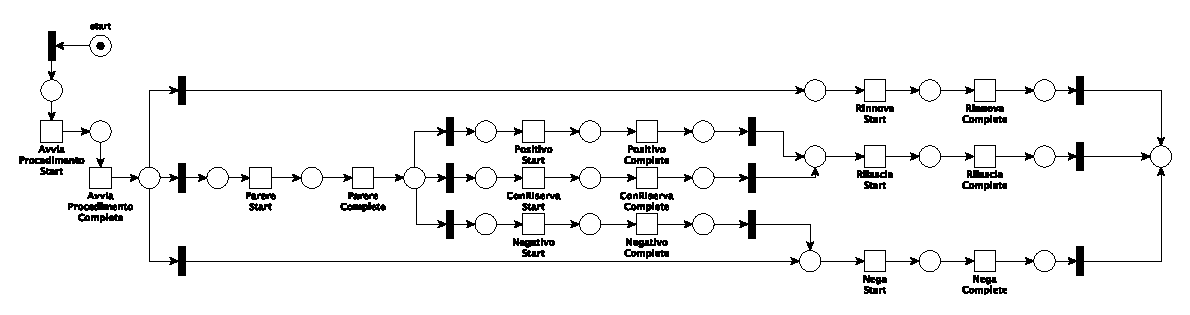
\includegraphics[scale=0.60]{./fig/animazioneconf/ConfPN}
%  \end{center}
%
%  
%\end{frame}
%\begin{frame}{Animazione Conformance}
% 
%  
%  \begin{center}
%   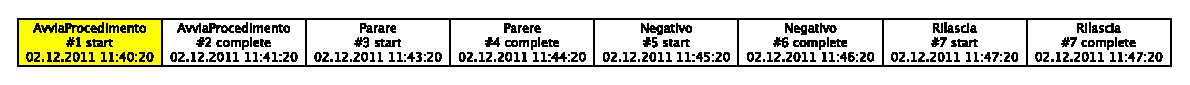
\includegraphics[scale=0.60]{./fig/animazioneconf/log1}\\[10pt]
%    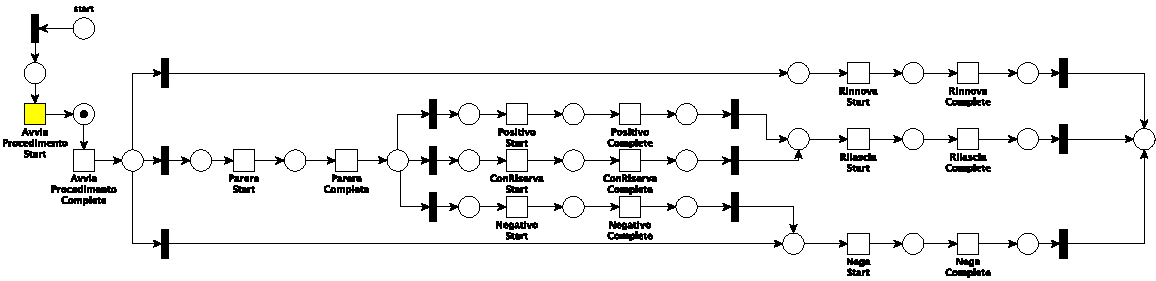
\includegraphics[scale=0.60]{./fig/animazioneconf/ConfPN1}
%  \end{center}
%
%  
%\end{frame}
%\begin{frame}{Animazione Conformance}
% 
%  
%  \begin{center}
%   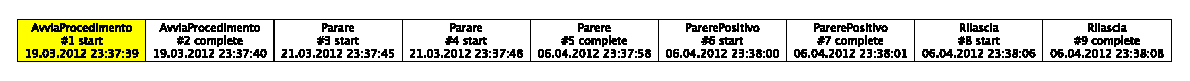
\includegraphics[scale=0.60]{./fig/animazioneconf/log2}\\[10pt]
%    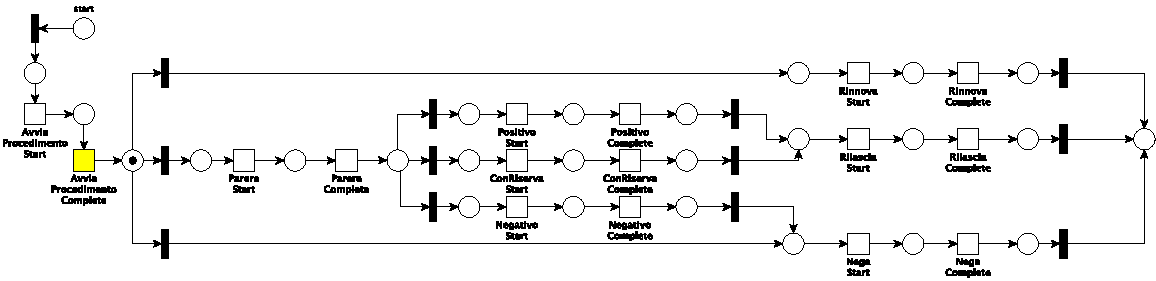
\includegraphics[scale=0.60]{./fig/animazioneconf/ConfPN2}
%  \end{center}
%
%  
%\end{frame}

\begin{frame}{Animazione Conformance}

%\multiinclude[format=eps,graphics={scale=0.6}]{./fig/animazioneconf/ConfPN}
\foreach \i in {0,1,2,3}%
        {%
		\only<\i>{%
		\includegraphics<\i>[scale=0.6]{./fig/animazioneconf/log\i}\\[10pt]
		\includegraphics<\i>[scale=0.6]{./fig/animazioneconf/ConfPN-\i}%
		}%end only
        }%end foreach

\end{frame}


	% ***AC \frame{
  \begin{block}{Esempio Calcolo Performance}
    
    \begin{itemize}
      \item Eventi del log $(A, 1s), (B, 2s), (C, 4), (D, 8s)$ 
      \item Sequenza di transizioni del log replay  $A, B, C, t1, D$
      \item Risultato della sequenza \textquotedblleft eager\textquotedblright $A, B, t1, C, D$
    \end{itemize}

  \end{block}
  \begin{center}
    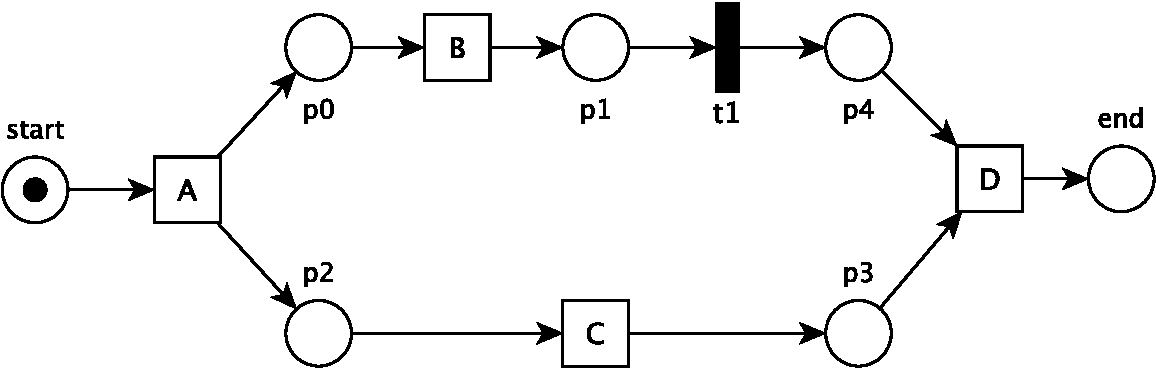
\includegraphics[scale=0.30]{./fig/LogReplay3a}
  \end{center}
  \begin {block}{Misure}
    \begin{tabular}{ccc}
                  \\
       $\TSync$   \\
       $\TTot$    \\
    \end{tabular}
  \end{block}
}

\frame{
  \begin{block}{Esempio Calcolo Performance}
    
    \begin{itemize}
      \item Eventi del log $\alert{(A, 1s)}, (B, 2s), (C, 4), (D, 8s)$ 
      \item Sequenza di transizioni del log replay  $A, B, C, t1, D$
      \item Risultato della sequenza \textquotedblleft eager\textquotedblright $\alert{A}, B, t1, C, D$
    \end{itemize}

  \end{block}
  \begin{center}
    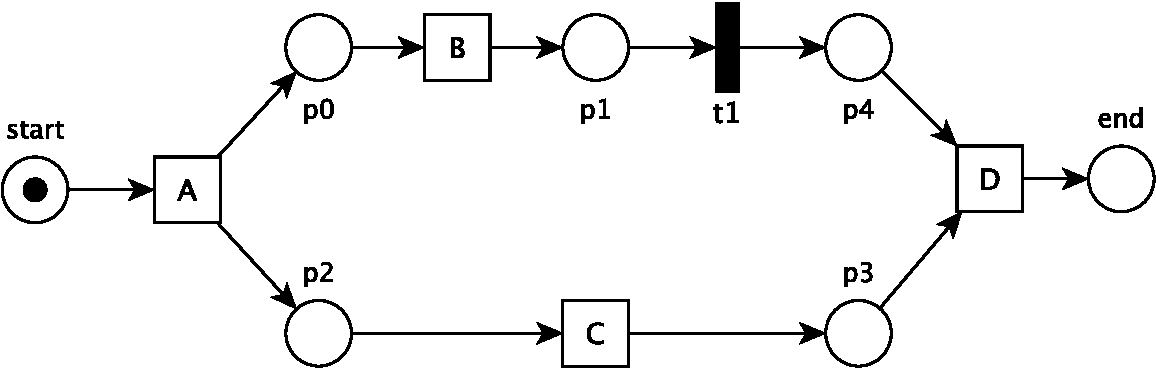
\includegraphics[scale=0.30]{./fig/LogReplay3a}
  \end{center}
  \begin {block}{Misure}
    \begin{tabular}{ccc}
                  \\
       $\TSync$   \\
       $\TTot$    \\
    \end{tabular}
  \end{block}
}

\frame{
  \begin{block}{Esempio Calcolo Performance}
    
    \begin{itemize}
      \item Eventi del log $\alert{(A, 1s)}, (B, 2s), (C, 4), (D, 8s)$ 
      \item Sequenza di transizioni del log replay  $A, B, C, t1, D$
      \item Risultato della sequenza \textquotedblleft eager\textquotedblright $\alert{A}, B, t1, C, D$
    \end{itemize}

  \end{block}
  \begin{center}
    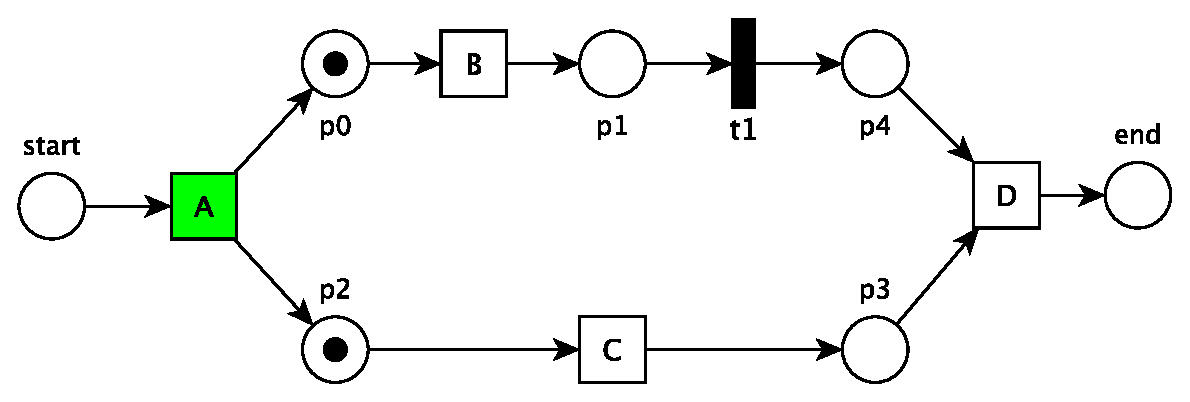
\includegraphics[scale=0.30]{./fig/LogReplay3b}
  \end{center}
  \begin {block}{Misure}
    \begin{tabular}{ccc}
                  & p0 & p2 \\
       $\TSync$   & 0  & 0  \\
       $\TTot$    &    &    \\
    \end{tabular}
  \end{block}
}
\frame{
  \begin{block}{Esempio Calcolo Performance}
    
    \begin{itemize}
      \item Eventi del log $(A, 1s), \alert{(B, 2s)}, (C, 4), (D, 8s)$ 
      \item Sequenza di transizioni del log replay  $A, B, C, t1, D$
      \item Risultato della sequenza \textquotedblleft eager\textquotedblright $A, \alert{B}, t1, C, D$
    \end{itemize}

  \end{block}
  \begin{center}
    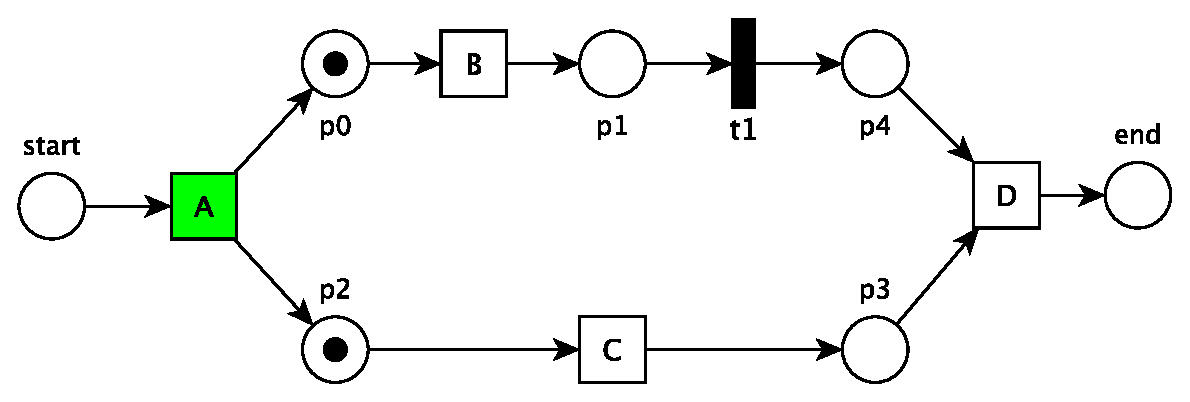
\includegraphics[scale=0.30]{./fig/LogReplay3b}
  \end{center}
  \begin {block}{Misure}
    \begin{tabular}{ccc}
                  & p0 & p2 \\
       $\TSync$   & 0  & 0  \\
       $\TTot$    &    &    \\
    \end{tabular}
  \end{block}
}
\frame{
  \begin{block}{Esempio Calcolo Performance}
    
    \begin{itemize}
      \item Eventi del log $(A, 1s), \alert{(B, 2s)}, (C, 4), (D, 8s)$ 
      \item Sequenza di transizioni del log replay  $A, B, C, t1, D$
      \item Risultato della sequenza \textquotedblleft eager\textquotedblright $A, \alert{B}, t1, C, D$
    \end{itemize}

  \end{block}
  \begin{center}
    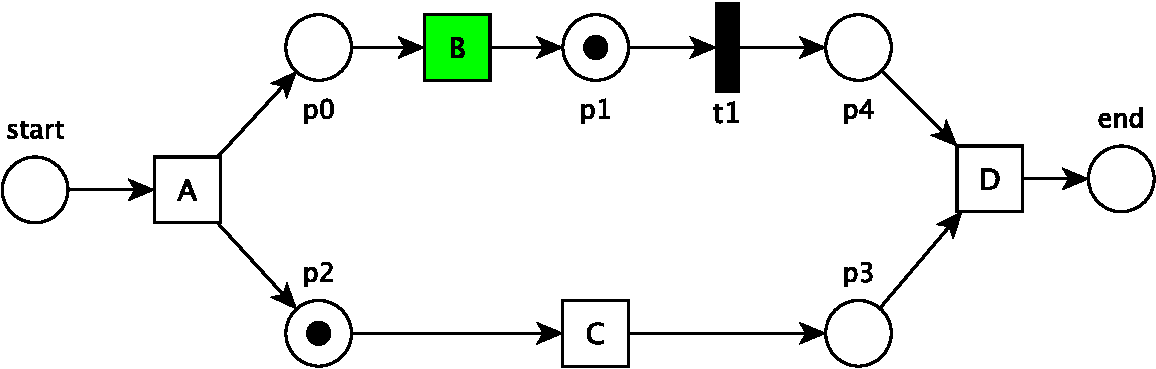
\includegraphics[scale=0.30]{./fig/LogReplay3c}
  \end{center}
  \begin {block}{Misure}
    \begin{tabular}{cccccc}
                  & p0 & p2 & p1 \\
       $\TSync$   & 0  & 0  & 0  \\
       $\TTot$    & 1  &    &    \\
    \end{tabular}
  \end{block}
}

% Attivazione di t1
\frame{
  \begin{block}{Esempio Calcolo Performance}
    
    \begin{itemize}
      \item Eventi del log $(A, 1s), \alert{(B, 2s)}, (C, 4), (D, 8s)$ 
      \item Sequenza di transizioni del log replay  $A, B, C, t1, D$
      \item Risultato della sequenza \textquotedblleft eager\textquotedblright $A, B, \alert{t1}, C, D$
    \end{itemize}

  \end{block}
  \begin{center}
    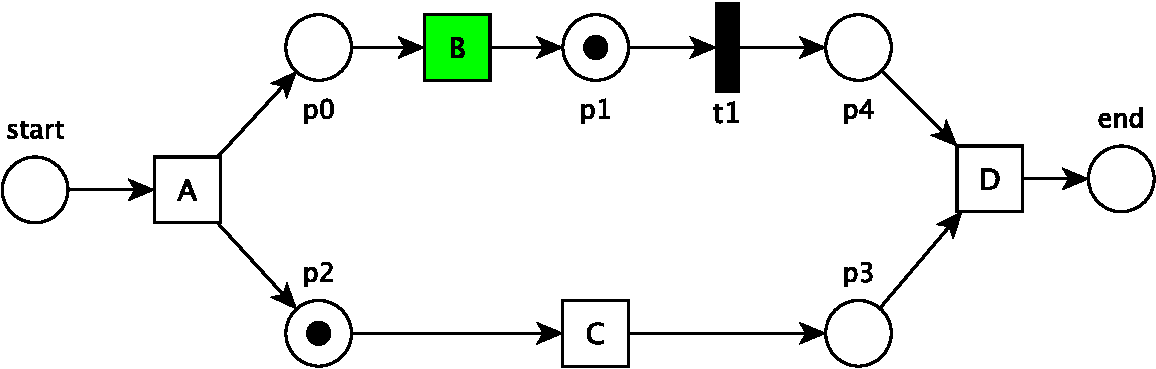
\includegraphics[scale=0.30]{./fig/LogReplay3c}
  \end{center}
  \begin {block}{Misure}
    \begin{tabular}{cccccc}
                  & p0 & p2 & p1 \\
       $\TSync$   & 0  & 0  & 0  \\
       $\TTot$    & 1  &    &    \\
    \end{tabular}
  \end{block}
}
\frame{
  \begin{block}{Esempio Calcolo Performance}
    
    \begin{itemize}
      \item Eventi del log $(A, 1s), \alert{(B, 2s)}, (C, 4), (D, 8s)$ 
      \item Sequenza di transizioni del log replay  $A, B, C, t1, D$
      \item Risultato della sequenza \textquotedblleft eager\textquotedblright $A, B, \alert{t1}, C, D$
    \end{itemize}
  \end {block}
  \begin{center}
    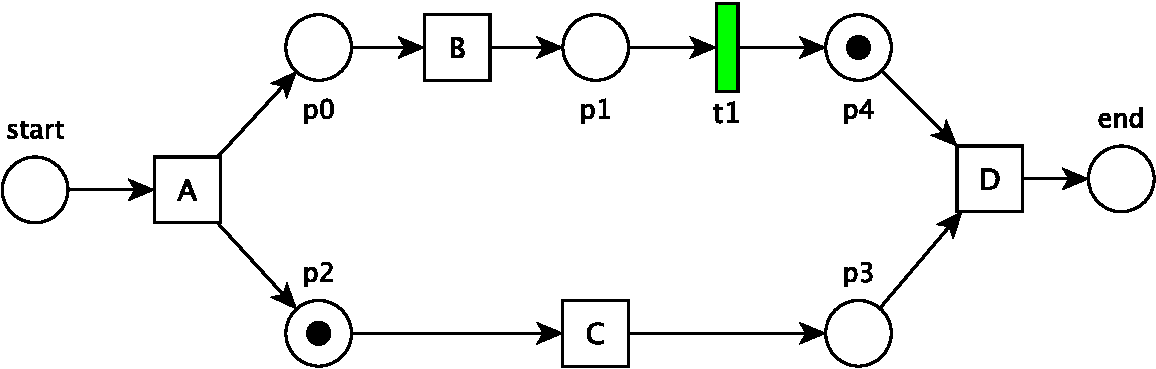
\includegraphics[scale=0.30]{./fig/LogReplay4d}
  \end{center}
  \begin {block}{Misure}
    \begin{tabular}{cccccc}
                  & p0 & p2 & p1 & p3 & p4 \\
       $\TSync$   & 0  & 0  & 0  &    &    \\
       $\TTot$    & 1  &    & 0  &    &    \\
    \end{tabular}
  \end{block}
}

\frame{
  \begin{block}{Esempio Calcolo Performance}
    
    \begin{itemize}
      \item Eventi del log $(A, 1s), (B, 2s), \alert{(C, 4)}, (D, 8s)$ 
      \item Sequenza di transizioni del log replay  $A, B, C, t1, D$
      \item Risultato della sequenza \textquotedblleft eager\textquotedblright $A, B, t1, \alert{C}, D$
    \end{itemize}
  \end {block}
  \begin{center}
    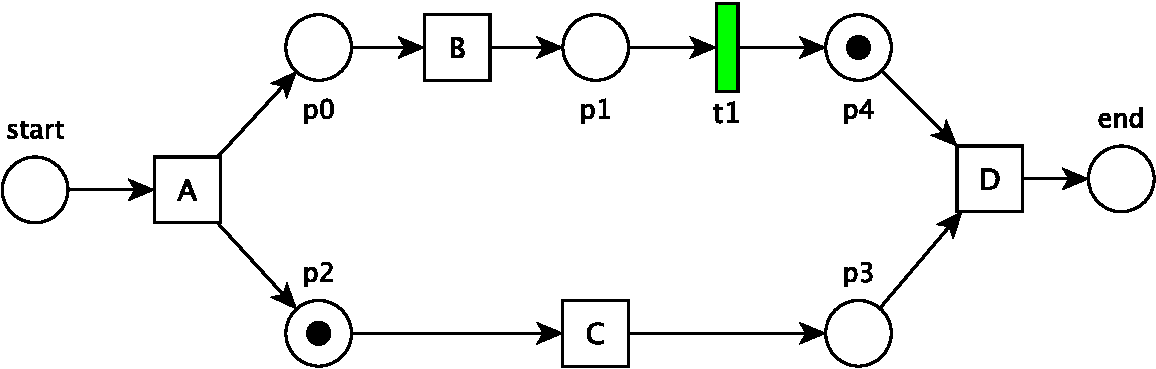
\includegraphics[scale=0.30]{./fig/LogReplay4d}
  \end{center}
  \begin {block}{Misure}
    \begin{tabular}{cccccc}
                  & p0 & p2 & p1 & p3 & p4 \\
       $\TSync$   & 0  & 0  & 0  &    &    \\
       $\TTot$    & 1  &    & 0  &    &    \\
    \end{tabular}
  \end{block}
}
\frame{
  \begin{block}{Esempio Calcolo Performance}
    
    \begin{itemize}
      \item Eventi del log $(A, 1s), (B, 2s), \alert{(C, 4)}, (D, 8s)$ 
      \item Sequenza di transizioni del log replay  $A, B, C, t1, D$
      \item Risultato della sequenza \textquotedblleft eager\textquotedblright $A, B, t1, \alert{C}, D$
    \end{itemize}
  \end {block}
  \begin{center}
    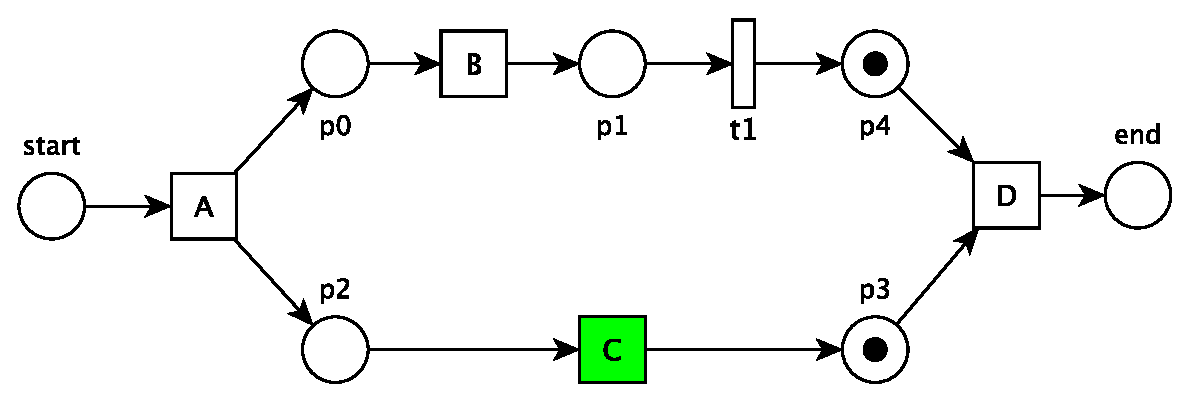
\includegraphics[scale=0.30]{./fig/LogReplay4e}
  \end{center}
  \begin {block}{Misure}
    \begin{tabular}{cccccc}
                  & p0 & p2 & p1 & p3 & p4 \\
       $\TSync$   & 0  & 0  & 0  & 0  & 2  \\
       $\TTot$    & 1  & 2  & 0  &    &    \\
    \end{tabular}
  \end{block}
}
\frame{
  \begin{block}{Esempio Calcolo Performance}
    
    \begin{itemize}
      \item Eventi del log $(A, 1s), (B, 2s), (C, 4), \alert{(D, 8s)}$ 
      \item Sequenza di transizioni del log replay  $A, B, C, t1, D$
      \item Risultato della sequenza \textquotedblleft eager\textquotedblright $A, B, t1, C, \alert{D}$
    \end{itemize}
  \end {block}
  \begin{center}
    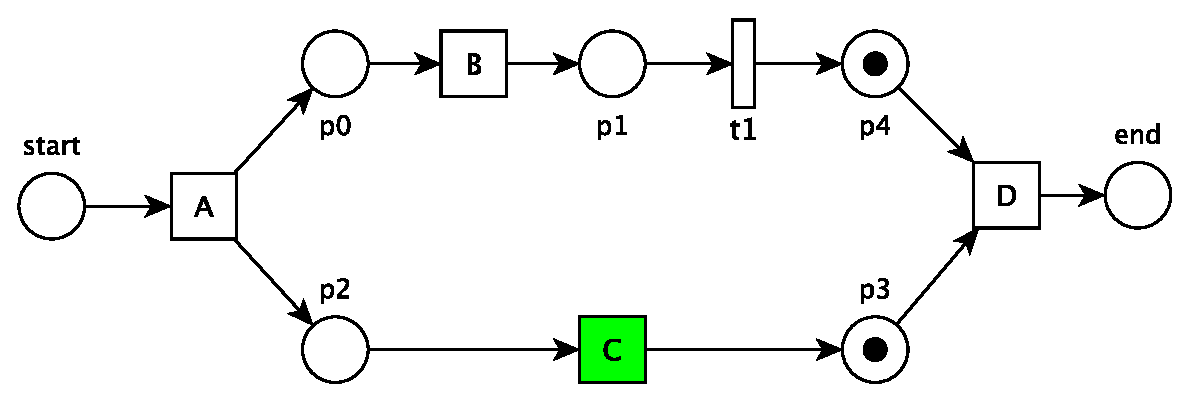
\includegraphics[scale=0.30]{./fig/LogReplay4e}
  \end{center}
  \begin {block}{Misure}
    \begin{tabular}{cccccc}
                  & p0 & p2 & p1 & p3 & p4 \\
       $\TSync$   & 0  & 0  & 0  & 0  & 2  \\
       $\TTot$    & 1  & 2  & 0  &   &   \\
    \end{tabular}
  \end{block}
}
\frame{
  \begin{block}{Esempio Calcolo Performance}
    
    \begin{itemize}
      \item Eventi del log $(A, 1s), (B, 2s), (C, 4), \alert{(D, 8s)}$ 
      \item Sequenza di transizioni del log replay  $A, B, C, t1, D$
      \item Risultato della sequenza \textquotedblleft eager\textquotedblright $A, B, t1, C, \alert{D}$
    \end{itemize}
  \end {block}
  \begin{center}
    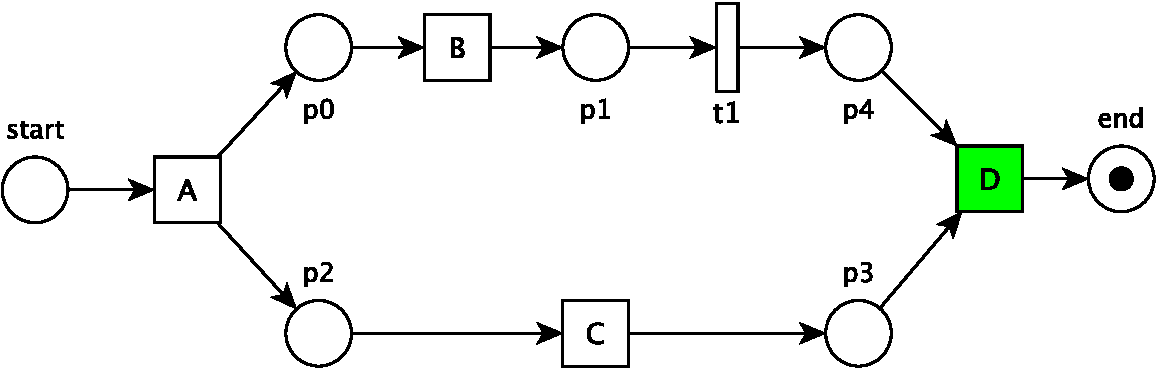
\includegraphics[scale=0.30]{./fig/LogReplay4f}
  \end{center}
  \begin {block}{Misure}
    \begin{tabular}{cccccc}
                  & p0 & p2 & p1 & p3 & p4 \\
       $\TSync$   & 0  & 0  & 0  & 0  & 2  \\
       $\TTot$    & 1  & 2  & 0  & 4  & 6  \\
    \end{tabular}
  \end{block}
}
%%% Local Variables: 
%%% mode: latex
%%% TeX-master: "main"
%%% End: 

	
	\begin{frame}{}
	  Esempio di analisi di conformance
	  \begin{center}
	    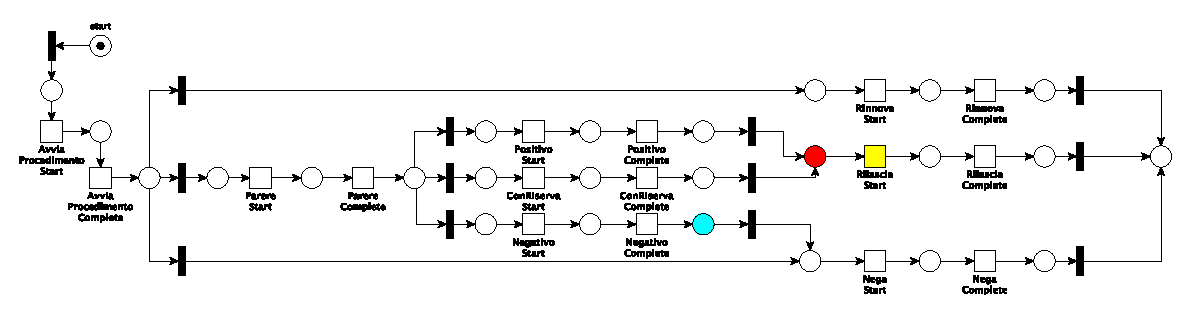
\includegraphics[scale=0.50]{./fig/animazioneconf/ConfPNfinal}\\[10pt]
	    
\includegraphics[scale=0.20]{./fig/animazioneconf/ConfPNz}\\[10pt]
	    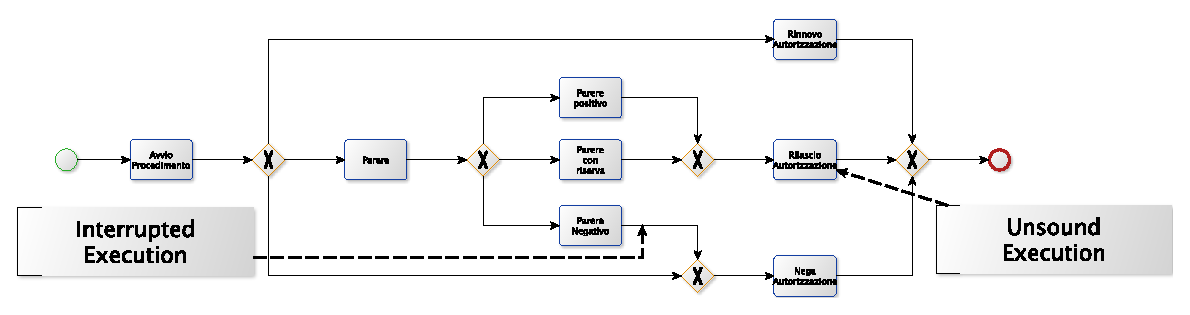
\includegraphics[scale=0.50]{./fig/animazioneconf/BPMNConf}
	  \end{center}
	\end{frame}
	
	\subsection{Proiezione dei risultati da Rete di Petri a BPMN}
	\begin{frame}{}
	  \begin{block}{Proiezione dei risultati di analisi su BPMN (Conformance)}
	    \begin{itemize}
	      \item \alert{Token mancanti}: Il log-replay produce token mancanti solo per eseguire transizioni visibili  $\Rightarrow$ pre-set di almeno una transizione visibile
	      \item \alert{Token rimanenti} Le transizioni invisibili sono eseguite solo se richiesto da una transizione visibile $\Rightarrow$ 
	        piazze nel  post-set di una transizione visibile  o di una transizione invisibile che produce pi\`{u} di un token
	
	    \end{itemize}
	  \end{block}
	  
	  \begin{center}
	    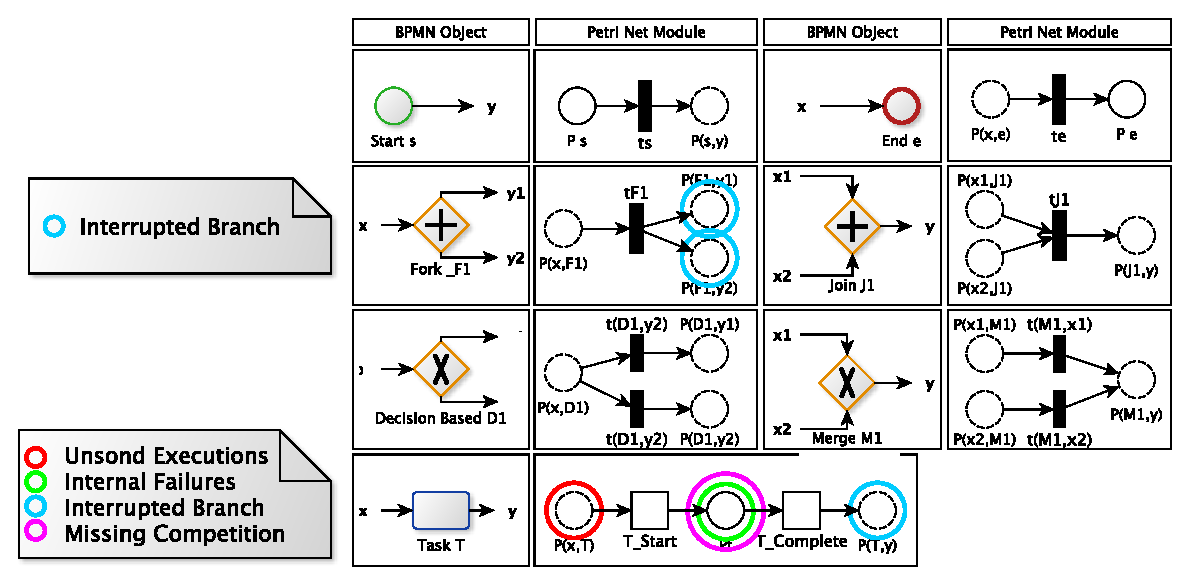
\includegraphics[scale=0.40]{./fig/MappingBPMNtoPN2}
	  \end{center}
	
	\end{frame}

	
\begin{frame}
	\frametitle{Classificazione dei dati di conformance}
	\begin{figure}
	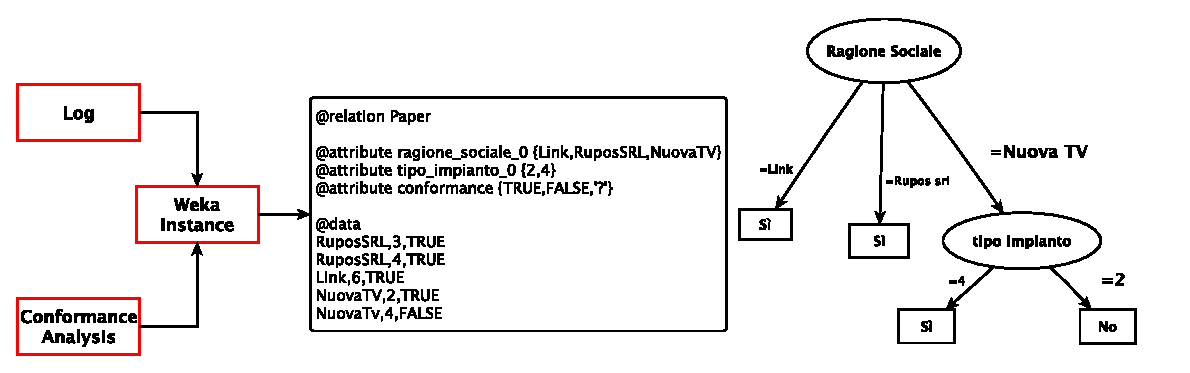
\includegraphics[scale=0.6]{./fig/animazioneconf/decisiontree1}
	\end{figure}
	\begin{block}{}
	\begin{itemize}
	\item Alcune istanze non sono conformi al modello: es. la transizione \textit{avvia istruttoria complete} \`{e} stato eseguito due volte.
	\item Le procedure del tipo impianto due dei processi di NuovaTV non rispettano il modello.
	\end{itemize}
	\end{block}
	\end{frame}
	
%	\begin{frame}
%	\frametitle{Possibili misure correttive}
%	\begin{block}{A livello di processo}
%	Riorganizzazione del processo aziendale: giudicare ragionevole saltare le fasi di valutazione per i clienti consolidati.
%	\end{block}
%	\begin{figure}
%	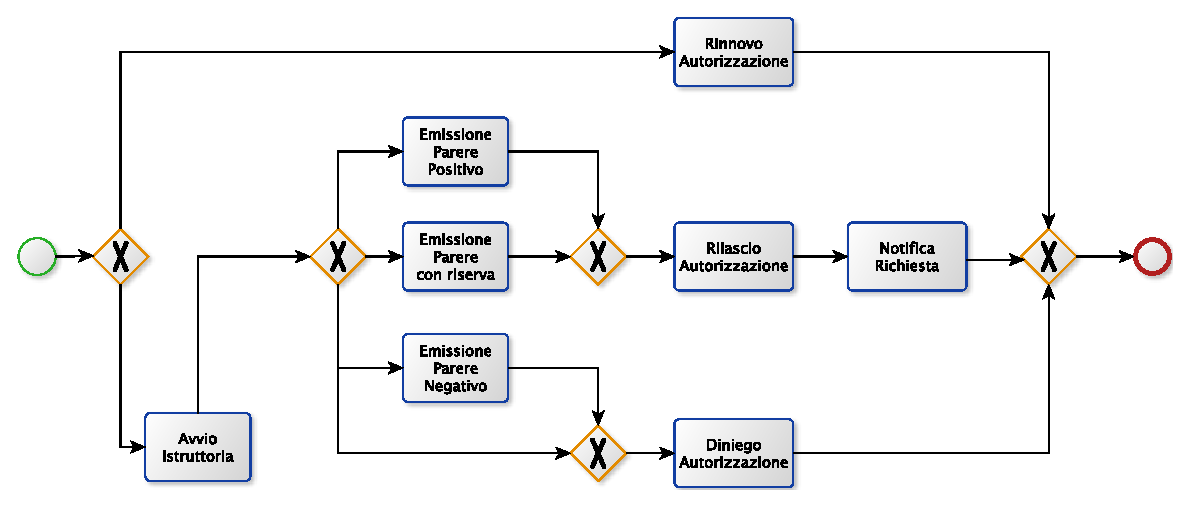
\includegraphics[scale=0.4]{./fig/BPMN}
%	\end{figure}
%	\begin{block}{Predizione}
%	Uso del classificatore in senso predittivo: prevedere i casi di non conformit\`{a} con segnalazione al personale per evitare errori noti.  
%	\end{block}
%	\end{frame}
		
	
	
	\frame{
	  Esempio di analisi di performance
	  \begin{center}
	    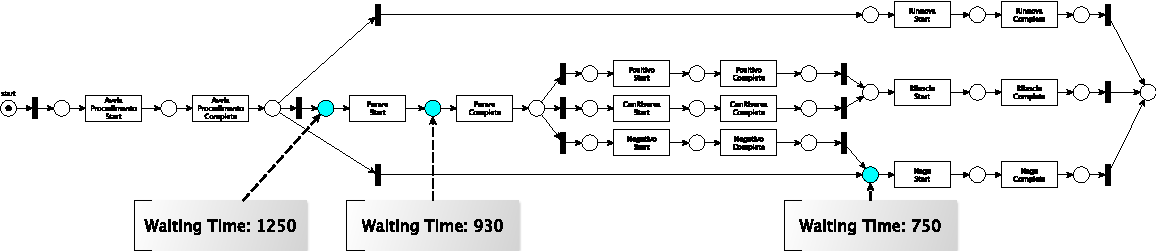
\includegraphics[scale=0.55]{./fig/PerfPN}\\[10pt]
	    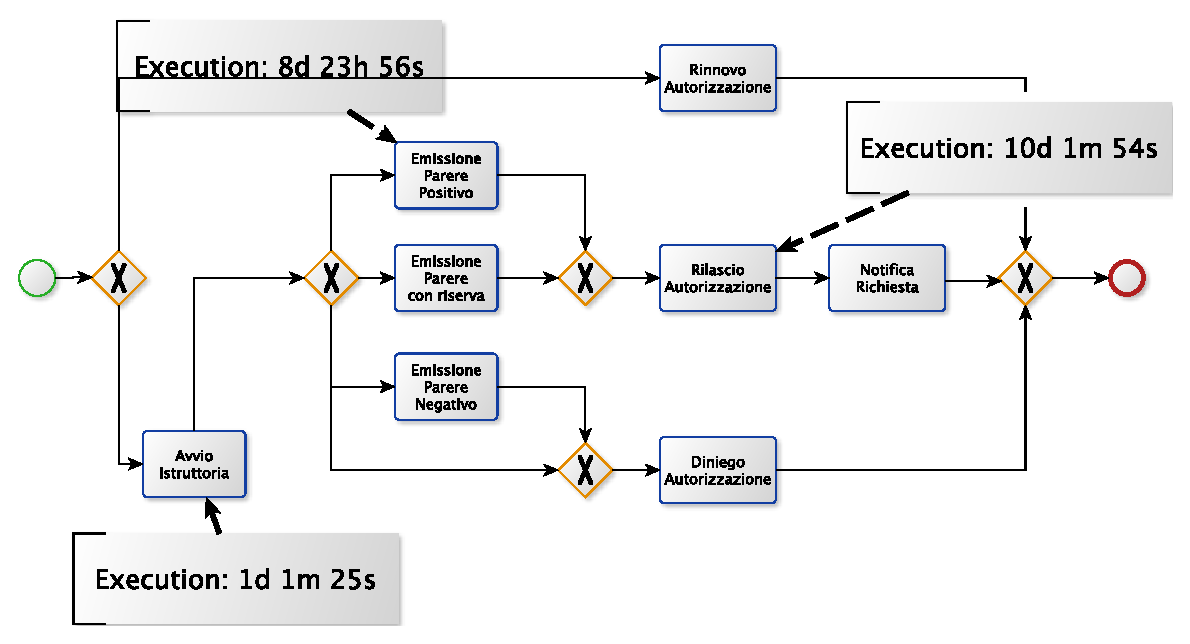
\includegraphics[scale=0.50]{./fig/BPMNPerf}
	  \end{center}
	}
	
	
	
	\frame{
	  \begin{block}{Proiezione dei risultati di analisi su BPMN (Performance)}
	    \begin{itemize}
	      \item \alert{Tempo di attesa}: transizioni invisibili eseguite immediatamente $\Rightarrow$ pre-set di transizioni visibili
	      \item \alert{Tempo di sincronizzazione} piazze che hanno almeno una transizione nel loro  post-set che dipende da un'altra piazza
	    \end{itemize}
	  \end{block}
	  \begin{center}
	    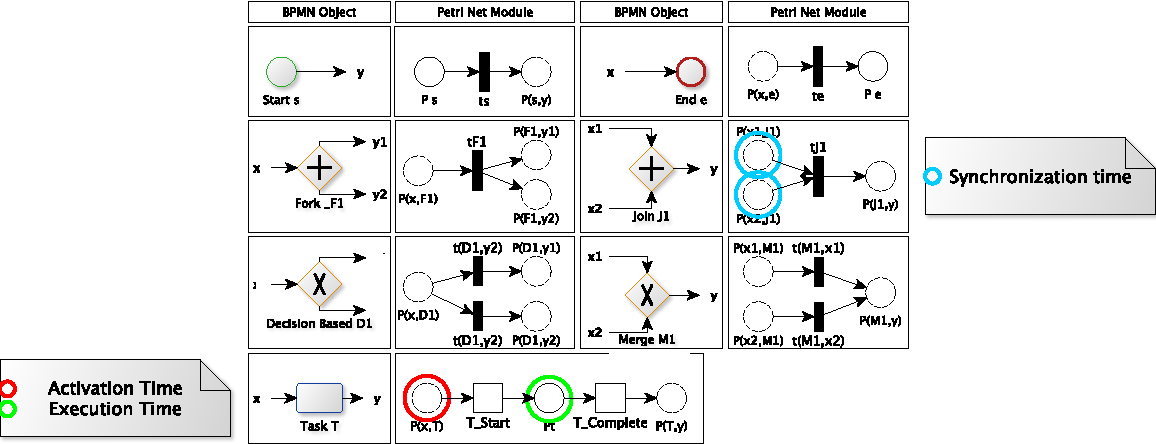
\includegraphics[scale=0.50]{./fig/MappingBPMNtoPN3}
	  \end{center}
	}
	
	%% \begin{frame}{[A2.3] Middleware prototipale}
	
	
	
	%% \end{frame}
	
	\section{ Middleware prototipale}
	%\section{Concluding Remarks}
	\frame{
	  \begin{block}{Middleware prototipale}
	    \begin{itemize}
	      \item Raffinamento dell'algoritmo di log-replay per una migliore gestione delle transizioni invisibili
	      \item Metodologia per proiettare misure di analisi sul modello BPMN
	      \item Nuovo contesto ProM per eseguire plugin in ambiente senza GUI
	    \item Plugin per trasformazione di sequence di eventi in sequenze eager
	    \item Plugin per  valutazione di performance di una Rete di Petri
	    \end{itemize}
	  \end{block}
	  \begin{block}<2->{Middleware prototipale: rilasci ad oggi}
	    \begin{itemize}
	        \item Plugin per trasformazione di Modelli BPMN in Reti di Petri
	        \item Plugin per proiezione di misure di analisi sul modello BPMN originale
	    \end{itemize}
	  \end{block}
	  \begin{block}<3->{Middleware prototipale: sviluppi in corso}
	    \begin{itemize}
	    \item Estensione della traduzione BPMN -- Rete di Petri con gestione di ciclo di vita di task con eventi intermedi
	    \item Integrazione nella piattaforma di toolkits di Data Mining
	    \end{itemize}
	  \end{block}
	}
	%\frame{\tableofcontents}
	
\appendix	

\frame{
	  \begin{block}{Da messaggi SOAP a eventi/transizioni della Rete di Petri }
	  \begin{center}
	  \begin{tiny}
	    \begin{tabular}{|l|lll|}
	      \hline
	      \textbf{Messaggi SOAP} & \textbf{Eventi BPMN} &  &\\
	
	      \hline
	      richiestaAutorizzazione & AvvioProcedimento & AvvioProcedimento
	      & \\
	      request  &  start &  complete &\\
	
	      \hline
	      interrogaStatoAutorizzazione & RinnovaAutorizzazione &
	      RinnovaAutorizzazione  & \\
	      response[Rinnovo] & start & complete &\\
	
	      \hline
	      interrogaStatoAutorizzazione & RilascioAutorizzazione &
	      RilascioAutorizzazione & \\
	      response[Rilascio] & start & complete & \\
	
	      \hline
	      interrogaStatoAutorizzazione & RilascioAutorizzazione &
	      NegaAutorizzazione & \\
	      response[Nega] & start & complete & \\
	
	      \hline
	      richiestaParere & Parere &  & \\
	      request & start & & \\
	
	      \hline
	      emissioneParere & Parere & ParereNegativo & ParereNegativo \\
	      request[Negativo] & complete & start & complete\\
	
	      \hline
	      emissioneParere & Parere & ParerePositivo & ParerePositivo \\
	      request[Positivo] & complete & start & complete\\
	
	      \hline
	      emissioneParere & Parere & ParereConRiserva & ParereConRiserva \\
	      request[conRiserva] & complete & start & complete\\
	
	      \hline
	    \end{tabular}
	  \end{tiny}
	  \end{center}
	
	  \end{block}
	
	}
%%\subsection{Tecniche di analisi}
%	\frame{
%	  \begin{block}{Tecniche di analisi di Reti di Petri adottate}
%	    
%	    \begin{itemize}
%	      \item I log delle istanze di processi sono sequenze ordinate di eventi (e.g. in base a timestamp)
%	      \item Gli eventi dei log sono mappati su transizioni della rete
%	      \item<2-> Algoritmo di \alert{log-replay}: ri-esegue un log di una istanza di processo in modo ``non bloccante''
%	        
%	        \begin{enumerate}
%	          \item Si mette un token nella piazza di partenza
%	          \item Se estrae il primo evento del log
%	          \item Si esegue la transizione corrispondente
%	            \begin{itemize}
%	              \item se la transizione non \`{e} abilitata vengono creati artificialmente i token mancanti
%	            \end{itemize}
%	        \end{enumerate}
%	      \item <3->Metriche calcolate durante il log-replay
%	        \begin{itemize}
%	          \item Numero di token mancanti o rimanenti per ogni piazza o transizione
%	          \item Numero di attraversamenti per ogni arco
%	          \item Tempo di soggiorno/attesa/sincronizzazione per ogni piazza
%	        \end{itemize}
%	    \end{itemize}
%	
%	  \end{block}
%	}
%	
%	% \frame{
  \begin{block}{Log-replay examples}
    Trace log $(A, 1s), (B, 2s), (C, 4s), (D, 8s)$ 
  \end{block}
  \begin{center}
    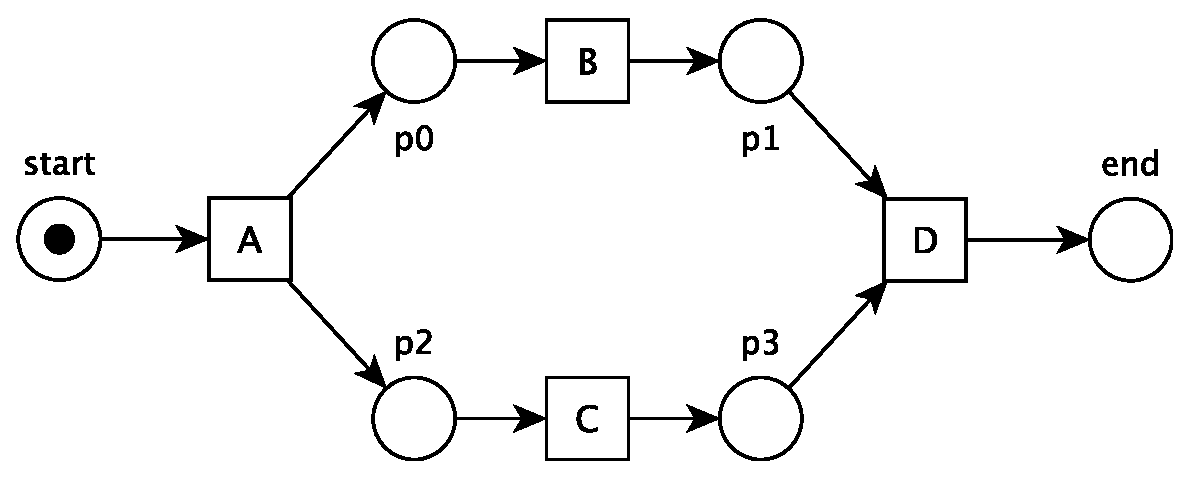
\includegraphics[scale=0.30]{./fig/LogReplay1a}
  \end{center}
  \begin {block}{Measures}
    \begin{tabular}{cc}
    \end{tabular}
  \end{block}
}
\frame{
  \begin{block}{Log-replay examples}
    Trace log $\alert{(A, 1s)}, (B, 2s), (C, 4s), (D, 8s)$ 
  \end{block}
  \begin{center}
    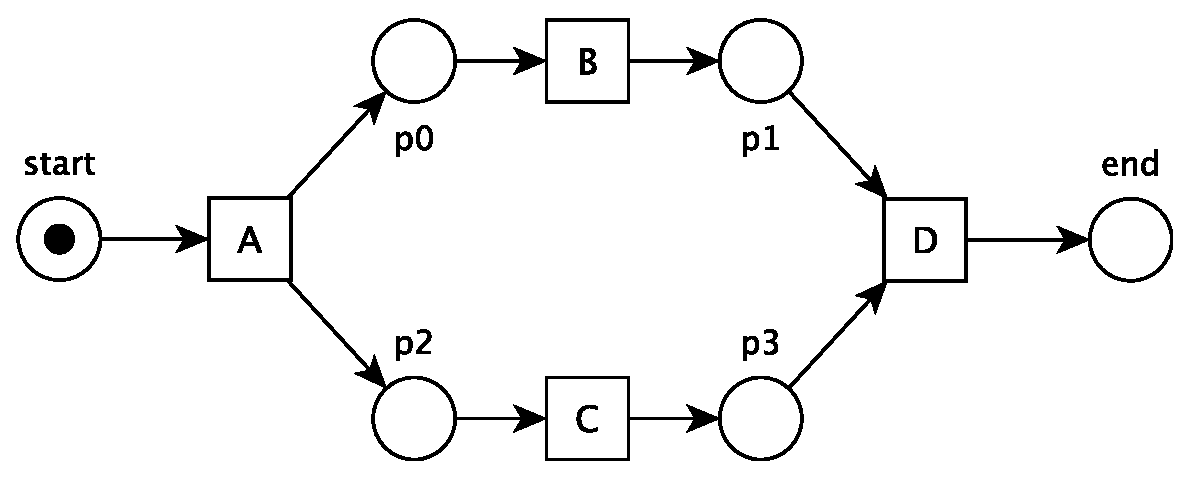
\includegraphics[scale=0.30]{./fig/LogReplay1a}
  \end{center}
  \begin {block}{Measures}
    \begin{tabular}{cc}
    \end{tabular}
  \end{block}
}
\frame{
  \begin{block}{Log-replay examples}
    Trace log $\alert{(A, 1s)}, (B, 2s), (C, 4s), (D, 8s)$ 
  \end{block}
  \begin{center}
    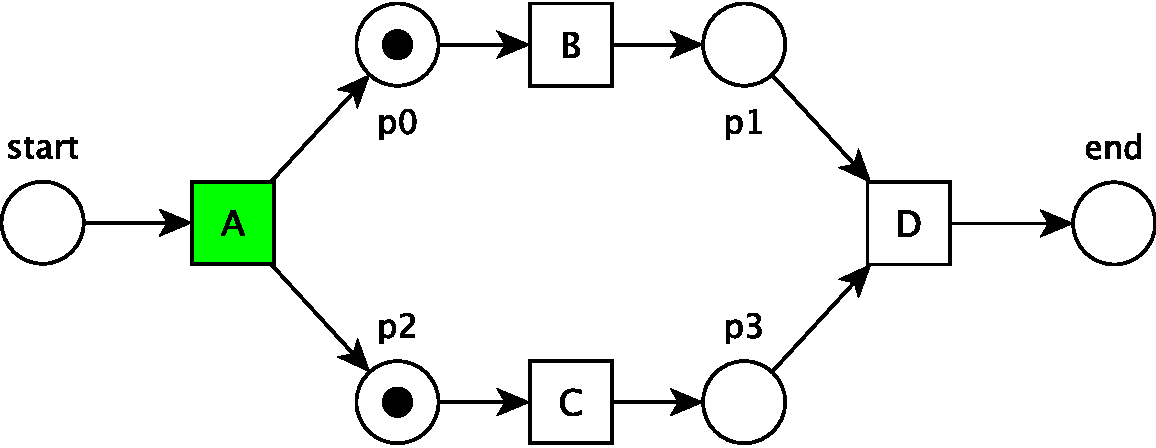
\includegraphics[scale=0.30]{./fig/LogReplay1b}
  \end{center}
  \begin {block}{Measures}
    \begin{tabular}{ccc}
                  & p0 & p2 \\
       $\TSync$   & 0  & 0  \\
    \end{tabular}
  \end{block}
}
\frame{
  \begin{block}{Log-replay examples}
    Trace log $(A, 1s), \alert{(B, 2s)}, (C, 4s), (D, 8s)$ 
  \end{block}
  \begin{center}
    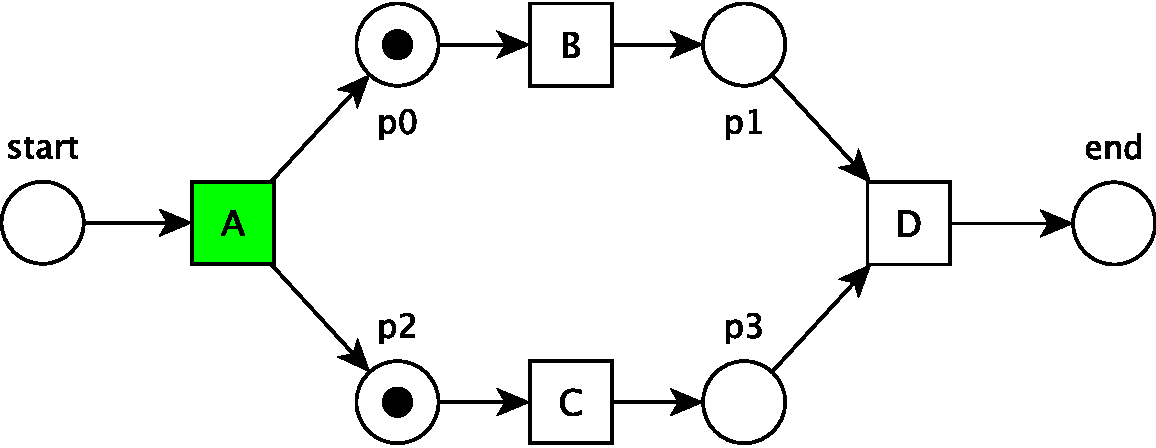
\includegraphics[scale=0.30]{./fig/LogReplay1b}
  \end{center}
  \begin {block}{Measures}
    \begin{tabular}{ccc}
                  & p0 & p2 \\
       $\TSync$   & 0  & 0  \\
    \end{tabular}
  \end{block}
}
\frame{
  \begin{block}{Log-replay examples}
    Trace log $(A, 1s), \alert{(B, 2s)}, (C, 4s), (D, 8s)$ 
  \end{block}
  \begin{center}
    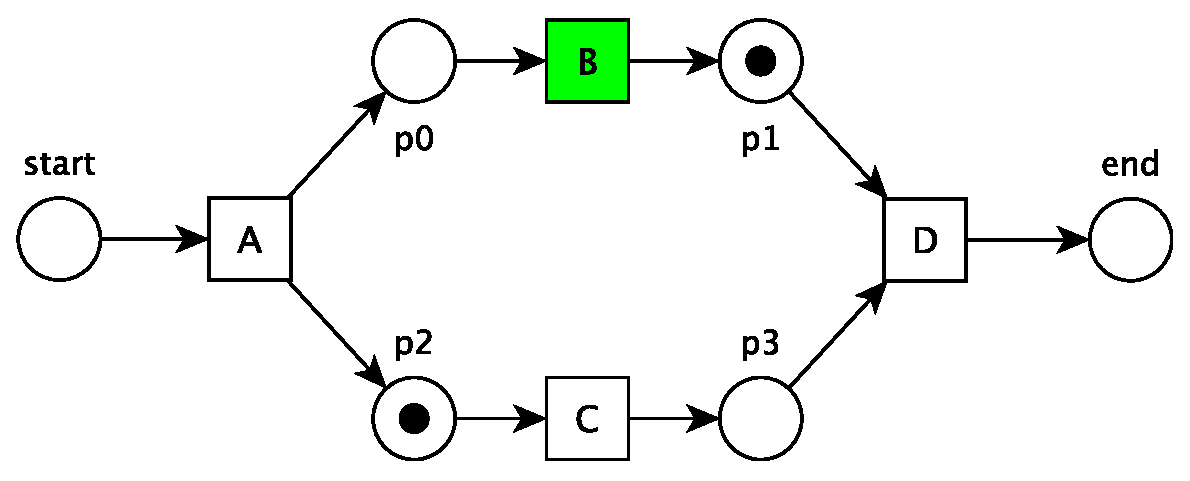
\includegraphics[scale=0.30]{./fig/LogReplay1c}
  \end{center}
  \begin {block}{Measures}
    \begin{tabular}{ccc}
                  & p0 & p2 \\
       $\TSync$   & 0  & 0  \\
       $\TTot$    & 1  &    \\
    \end{tabular}
  \end{block}
}
\frame{
  \begin{block}{Log-replay examples}
    Trace log $(A, 1s), (B, 2s), \alert{(C, 4s)}, (D, 8s)$ 
  \end{block}
  \begin{center}
    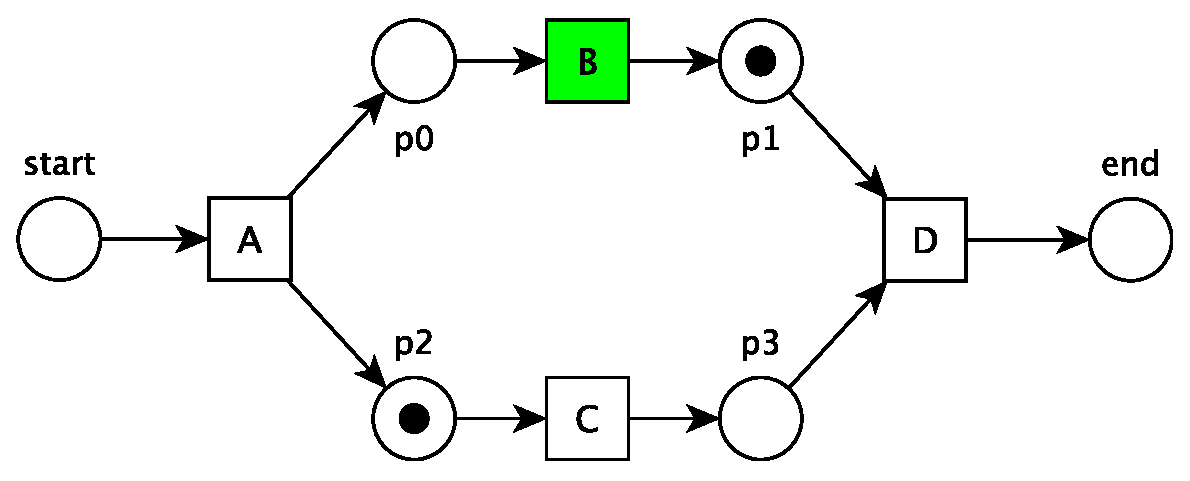
\includegraphics[scale=0.30]{./fig/LogReplay1c}
  \end{center}
  \begin {block}{Measures}
    \begin{tabular}{ccc}
                  & p0 & p2 \\
       $\TSync$   & 0  & 0  \\
       $\TTot$    & 1  &    \\
    \end{tabular}
  \end{block}
}
\frame{
  \begin{block}{Log-replay examples}
    Trace log $(A, 1s), (B, 2s), \alert{(C, 4s)}, (D, 8s)$ 
  \end{block}
  \begin{center}
    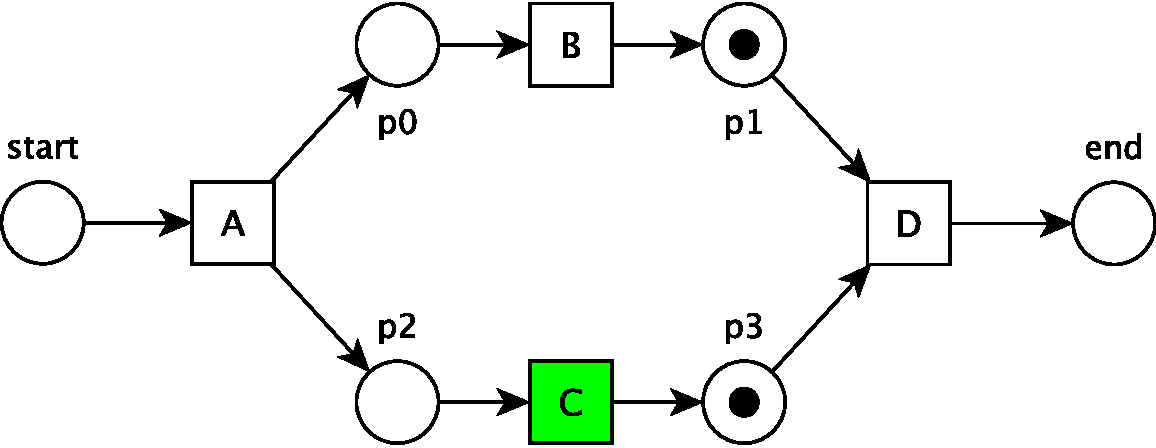
\includegraphics[scale=0.30]{./fig/LogReplay1d}
  \end{center}
  \begin {block}{Measures}
    \begin{tabular}{ccccccccc}
                  & p0 & p2 & p1 & p3 \\
       $\TSync$   & 0  & 0  & 2  & 0  \\
       $\TTot$    & 1  & 3  &    &    \\
    \end{tabular}
  \end{block}
}
\frame{
  \begin{block}{Log-replay examples}
    Trace log $(A, 1s), (B, 2s), (C, 4s), \alert{(D, 8s)}$ 
  \end{block}
  \begin{center}
    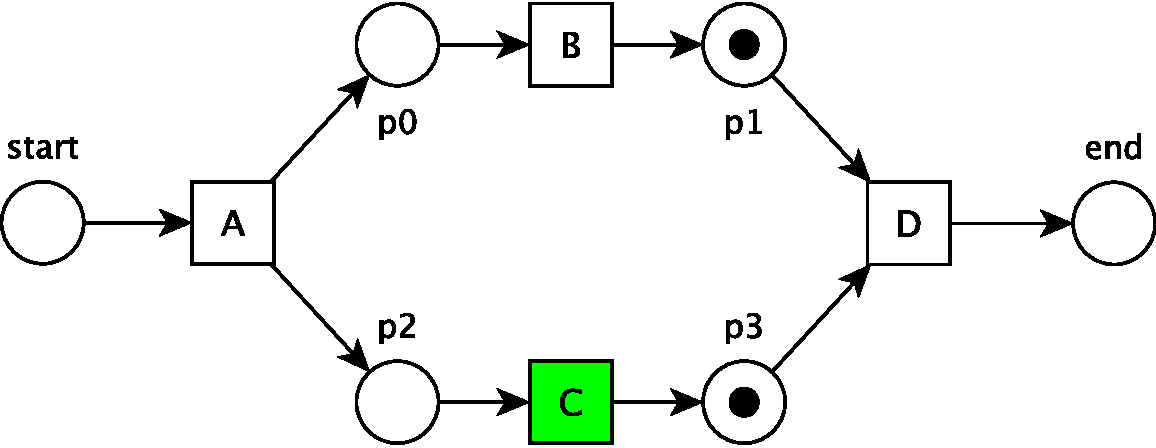
\includegraphics[scale=0.30]{./fig/LogReplay1d}
  \end{center}
  \begin {block}{Measures}
    \begin{tabular}{ccccccccc}
                  & p0 & p2 & p1 & p3 \\
       $\TSync$   & 0  & 0  & 2  & 0  \\
       $\TTot$    & 1  & 3  &    &    \\
    \end{tabular}
  \end{block}
}
\frame{
  \begin{block}{Log-replay examples}
    Trace log $(A, 1s), (B, 2s), (C, 4s), \alert{(D, 8s)}$ 
  \end{block}
  \begin{center}
    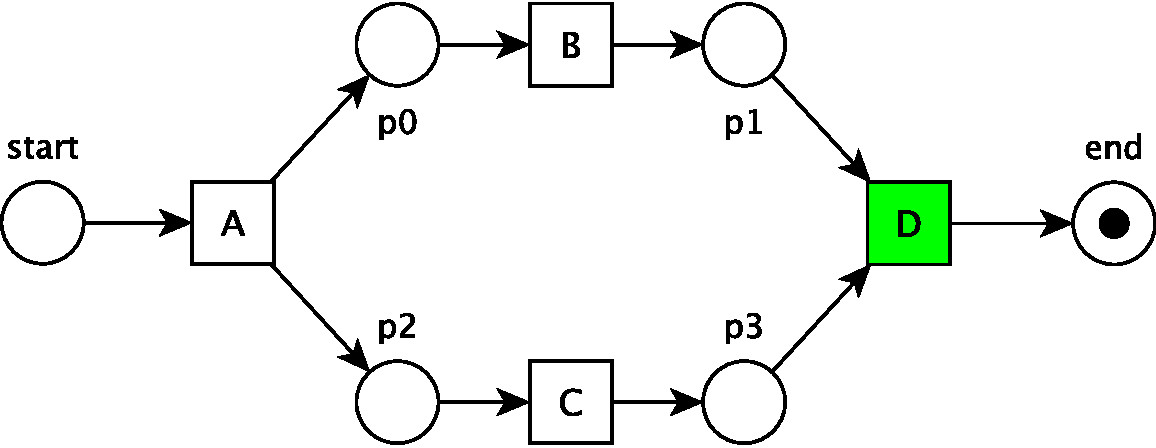
\includegraphics[scale=0.30]{./fig/LogReplay1e}
  \end{center}
  \begin {block}{Measures}
    \begin{tabular}{ccccccccc}
                  & p0 & p2 & p1 & p3 \\
       $\TSync$   & 0  & 0  & 2  & 0  \\
       $\TTot$    & 1  & 3  & 6  & 4  \\
    \end{tabular}
  \end{block}
}

%%% Local Variables: 
%%% mode: latex
%%% TeX-master: "main"
%%% End: 

%	% ***AC \frame{
  \begin{block}{Log-replay examples}
    Trace log $(A, 1s), (B, 2s), (D, 8s)$ 
  \end{block}
  \begin{center}
    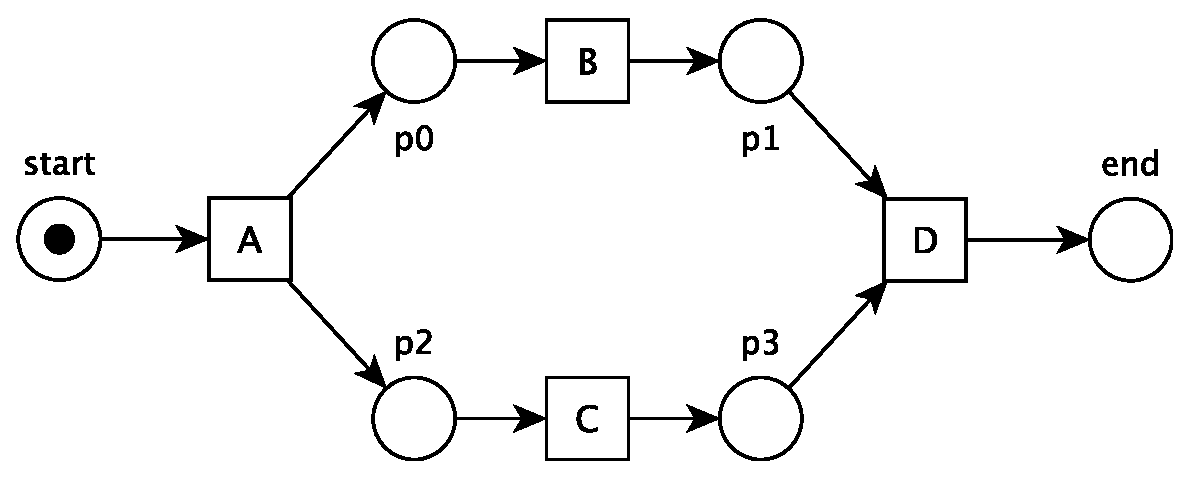
\includegraphics[scale=0.30]{./fig/LogReplay1a}
  \end{center}
  \begin {block}{Measures}
    \begin{tabular}{cc}
    \end{tabular}
  \end{block}
}
\frame{
  \begin{block}{Log-replay examples}
    Trace log $\alert{(A, 1s)}, (B, 2s), (D, 8s)$ 
  \end{block}
  \begin{center}
    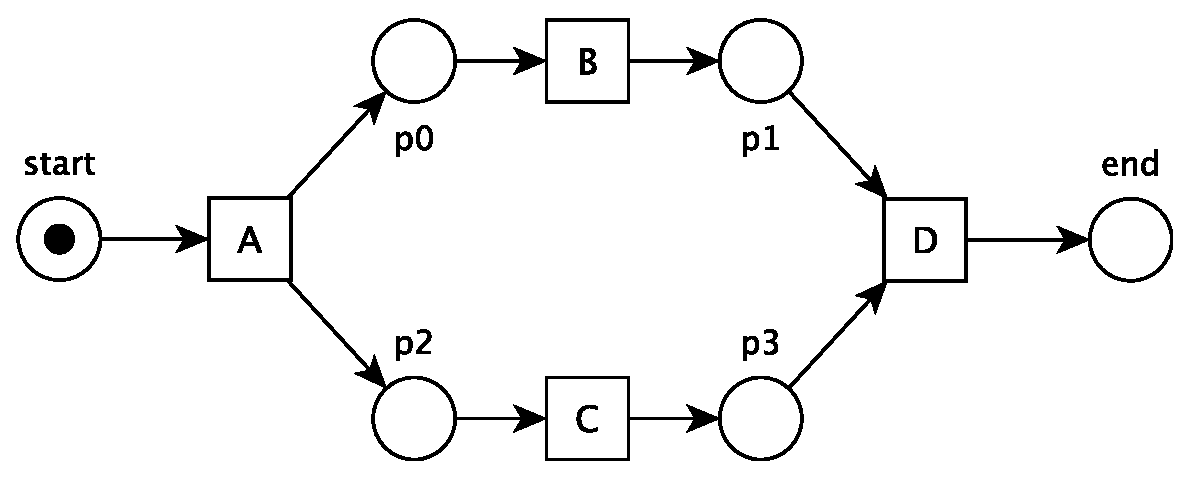
\includegraphics[scale=0.30]{./fig/LogReplay1a}
  \end{center}
  \begin {block}{Measures}
    \begin{tabular}{cc}
    \end{tabular}
  \end{block}
}
\frame{
  \begin{block}{Log-replay examples}
    Trace log $\alert{(A, 1s)}, (B, 2s), (D, 8s)$ 
  \end{block}
  \begin{center}
    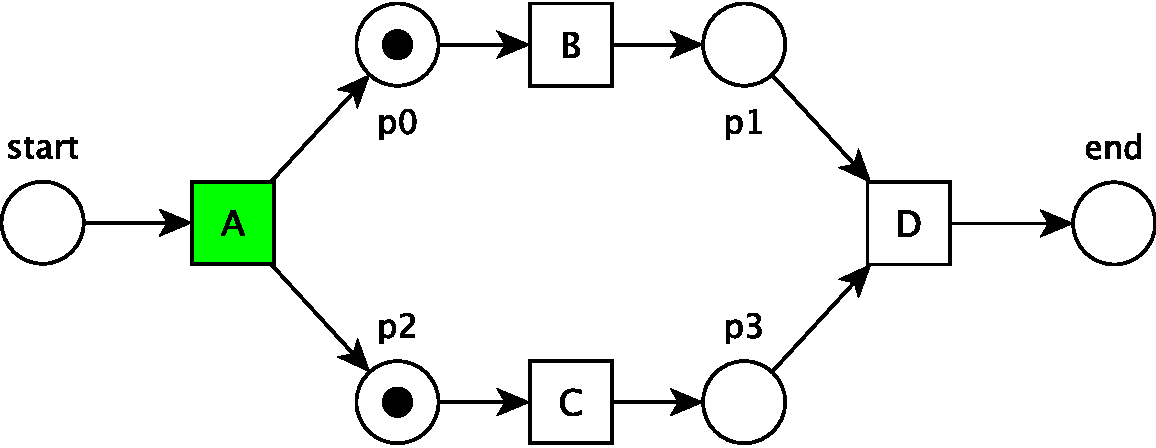
\includegraphics[scale=0.30]{./fig/LogReplay1b}
  \end{center}
  \begin {block}{Measures}
    \begin{tabular}{ccc}
                  & p0 & p2 \\
       $\TSync$   & 0  & 0  \\
    \end{tabular}
  \end{block}
}
\frame{
  \begin{block}{Log-replay examples}
    Trace log $(A, 1s), \alert{(B, 2s)}, (D, 8s)$ 
  \end{block}
  \begin{center}
    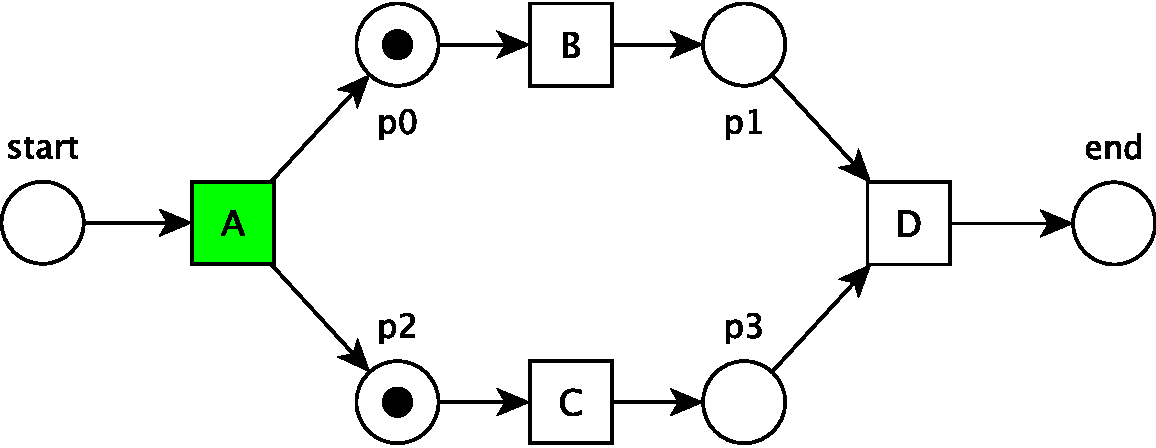
\includegraphics[scale=0.30]{./fig/LogReplay1b}
  \end{center}
  \begin {block}{Measures}
    \begin{tabular}{ccc}
                  & p0 & p2 \\
       $\TSync$   & 0  & 0  \\
    \end{tabular}
  \end{block}
}
\frame{
  \begin{block}{Log-replay examples}
    Trace log $(A, 1s), \alert{(B, 2s)}, (D, 8s)$ 
  \end{block}
  \begin{center}
    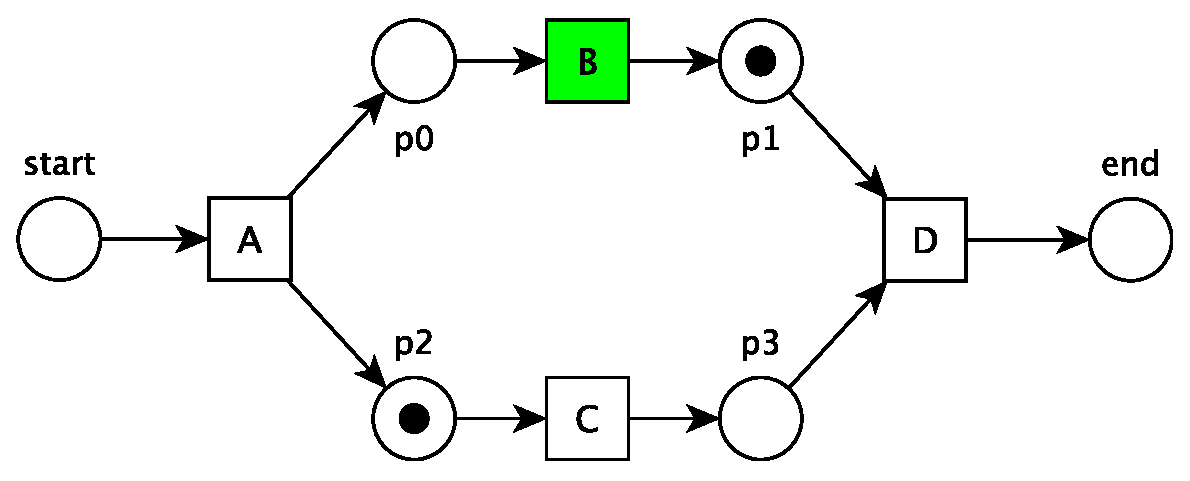
\includegraphics[scale=0.30]{./fig/LogReplay1c}
  \end{center}
  \begin {block}{Measures}
    \begin{tabular}{ccc}
                  & p0 & p2 \\
       $\TSync$   & 0  & 0  \\
       $\TTot$    & 1  &    \\
    \end{tabular}
  \end{block}
}
\frame{
  \begin{block}{Log-replay examples}
    Trace log $(A, 1s), (B, 2s), \alert{(D, 8s)}$ 
  \end{block}
  \begin{center}
    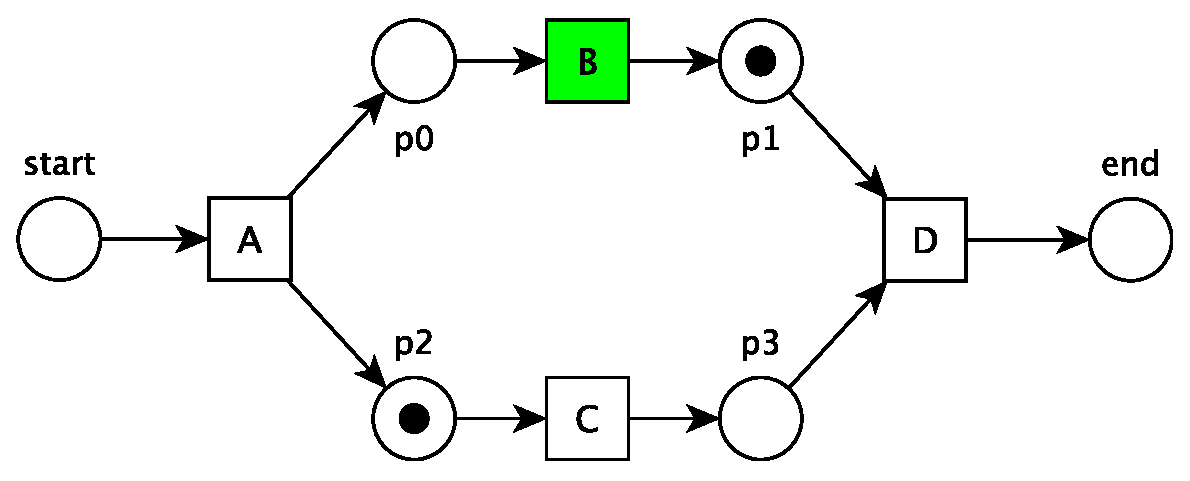
\includegraphics[scale=0.30]{./fig/LogReplay1c}
  \end{center}
  \begin {block}{Measures}
    \begin{tabular}{ccc}
                  & p0 & p2 \\
       $\TSync$   & 0  & 0  \\
       $\TTot$    & 1  &    \\
    \end{tabular}
  \end{block}
}

\frame{
  \begin{block}{Log-replay examples}
    Trace log $(A, 1s), (B, 2s), \alert{(D, 8s)}$ 
  \end{block}
  \begin{center}
    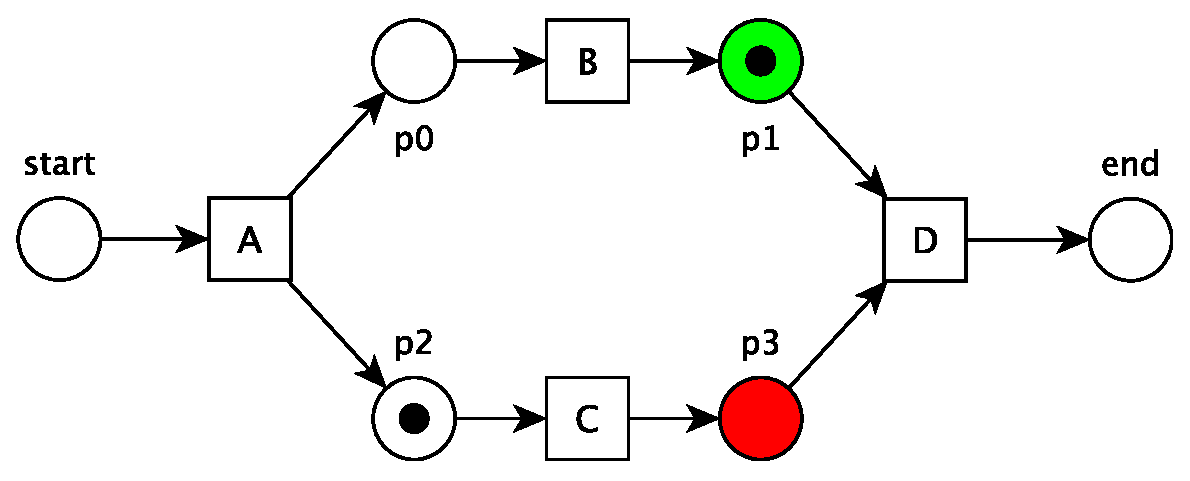
\includegraphics[scale=0.30]{./fig/LogReplay2d}
  \end{center}
  \begin {block}{Measures}
    \begin{tabular}{ccc}
                  & p0 & p2 \\
       $\TSync$   & 0  & 0  \\
       $\TTot$    & 1  &    \\
    \end{tabular}
  \end{block}
}
\frame{
  \begin{block}{Log-replay examples}
    Trace log $(A, 1s), (B, 2s), \alert{(D, 8s)}$ 
  \end{block}
  \begin{center}
    \includegraphics[scale=0.30]{./fig/LogReplay2f}
  \end{center}
  \begin {block}{Measures}
    \begin{tabular}{ccc}
                  & p0 & p2 \\
       $\TSync$   & 0  & 0  \\
       $\TTot$    & 1  &    \\
    \end{tabular}
    \begin{tabular}{ccc}
                  & p3 \\
       $Missing$  & 1  \\
    \end{tabular}
  \end{block}
}
\frame{
  \begin{block}{Log-replay examples}
    Trace log $(A, 1s), (B, 2s), \alert{(D, 8s)}$ 
  \end{block}
  \begin{center}
    \includegraphics[scale=0.30]{./fig/LogReplay2g}
  \end{center}
  \begin {block}{Measures}
    \begin{tabular}{ccc}
                  & p0 & p2 \\
       $\TSync$   & 0  & 0  \\
       $\TTot$    & 1  &    \\
    \end{tabular}
    \begin{tabular}{ccc}
                  & p3 \\
       $Missing$  & 1  \\
    \end{tabular}
  \end{block}
}
\frame{
  \begin{block}{Log-replay examples}
    Trace log $(A, 1s), (B, 2s), \alert{(D, 8s)}$ 
  \end{block}
  \begin{center}
    \includegraphics[scale=0.30]{./fig/LogReplay2h}
  \end{center}
  \begin {block}{Measures}
    \begin{tabular}{ccc}
                  & p0 & p2 \\
       $\TSync$   & 0  & 0  \\
       $\TTot$    & 1  &    \\
    \end{tabular}
    \begin{tabular}{ccc}
                   & p3 & p2 \\
       $Missing$   & 1  & 0  \\
       $Remaining$ & 0  & 1   \\
    \end{tabular}
  \end{block}
}


%%% Local Variables: 
%%% mode: latex
%%% TeX-master: "main"
%%% End: 

%	% \frame{
  \begin{block}{Log-replay examples}
    Trace log $\alert{(A, 1s)}, (B, 2s), (C, 4), (D, 8s)$ 
  \end{block}
  \begin{center}
    \includegraphics[scale=0.30]{./fig/LogReplay3a}
  \end{center}
  \begin {block}{Measures}
    \begin{tabular}{ccc}
                  \\
       $\TSync$   \\
       $\TTot$    \\
    \end{tabular}
  \end{block}
}
\frame{
  \begin{block}{Log-replay examples}
    Trace log $\alert{(A, 1s)}, (B, 2s), (C, 4), (D, 8s)$ 
  \end{block}
  \begin{center}
    \includegraphics[scale=0.30]{./fig/LogReplay3b}
  \end{center}
  \begin {block}{Measures}
    \begin{tabular}{ccc}
                  & p0 & p2 \\
       $\TSync$   & 0  & 0  \\
       $\TTot$    &    &    \\
    \end{tabular}
  \end{block}
}
\frame{
  \begin{block}{Log-replay examples}
    Trace log $(A, 1s), \alert{(B, 2s)}, (C, 4), (D, 8s)$ 
  \end{block}
  \begin{center}
    \includegraphics[scale=0.30]{./fig/LogReplay3b}
  \end{center}
  \begin {block}{Measures}
    \begin{tabular}{ccc}
                  & p0 & p2 \\
       $\TSync$   & 0  & 0  \\
       $\TTot$    &    &    \\
    \end{tabular}
  \end{block}
}
\frame{
  \begin{block}{Log-replay examples}
    Trace log $(A, 1s), \alert{(B, 2s)}, (C, 4), (D, 8s)$ 
  \end{block}
  \begin{center}
    \includegraphics[scale=0.30]{./fig/LogReplay3c}
  \end{center}
  \begin {block}{Measures}
    \begin{tabular}{cccccc}
                  & p0 & p2 & p1 \\
       $\TSync$   & 0  & 0  & 0  \\
       $\TTot$    & 1  &    &    \\
    \end{tabular}
  \end{block}
}

% Attivazione di C
\frame{
  \begin{block}{Log-replay examples}
    Trace log $(A, 1s), (B, 2s), \alert{(C, 4)}, (D, 8s)$ 
  \end{block}
  \begin{center}
    \includegraphics[scale=0.30]{./fig/LogReplay3c}
  \end{center}
  \begin {block}{Measures}
    \begin{tabular}{cccccc}
                  & p0 & p2 & p1 \\
       $\TSync$   & 0  & 0  & 0  \\
       $\TTot$    & 1  &    &    \\
    \end{tabular}
  \end{block}
}
\frame{
  \begin{block}{Log-replay examples}
    Trace log $(A, 1s), (B, 2s), \alert{(C, 4)}, (D, 8s)$ 
  \end{block}
  \begin{center}
    \includegraphics[scale=0.30]{./fig/LogReplay3d}
  \end{center}
  \begin {block}{Measures}
    \begin{tabular}{cccccc}
                  & p0 & p2 & p1 & p3 \\
       $\TSync$   & 0  & 0  & 0  &    \\
       $\TTot$    & 1  & 3  &    &    \\
    \end{tabular}
  \end{block}
}

% attivazione D
\frame{
  \begin{block}{Log-replay examples}
    Trace log $(A, 1s), (B, 2s), (C, 4), \alert{(D, 8s)}$ 
  \end{block}
  \begin{center}
    \includegraphics[scale=0.30]{./fig/LogReplay3d}
  \end{center}
  \begin {block}{Measures}
    \begin{tabular}{cccccc}
                  & p0 & p2 & p1 & p3 \\
       $\TSync$   & 0  & 0  & 0  &    \\
       $\TTot$    & 1  & 3  &    &    \\
    \end{tabular}
  \end{block}
}
\frame{
  \begin{block}{Log-replay examples}
    Trace log $(A, 1s), (B, 2s), (C, 4), \alert{(D, 8s)}$ 
  \end{block}
  \begin{center}
    \includegraphics[scale=0.30]{./fig/LogReplay3e}
  \end{center}
  \begin {block}{Measures}
    \begin{tabular}{cccccc}
                  & p0 & p2 & p1 & p3 & p4 \\
       $\TSync$   & 0  & 0  & 0  & 4  & 0  \\
       $\TTot$    & 1  & 3  & 6  &    &   \\
    \end{tabular}
  \end{block}
}
\frame{
  \begin{block}{Log-replay examples}
    Trace log $(A, 1s), (B, 2s), (C, 4), \alert{(D, 8s)}$ 
  \end{block}
  \begin{center}
    \includegraphics[scale=0.30]{./fig/LogReplay3f}
  \end{center}
  \begin {block}{Measures}
    \begin{tabular}{cccccc}
                  & p0 & p2 & p1 & p3 & p4 \\
       $\TSync$   & 0  & 0  & 0  & 4  & 0  \\
       $\TTot$    & 1  & 3  & 6  & 4  & 0 \\
    \end{tabular}
  \end{block}
}

%%% Local Variables: 
%%% mode: latex
%%% TeX-master: "main"
%%% End: 

%	
%	
%	\frame{
%	  \begin{block}{Un contributo originale: raffinamento dell'analisi di performance}
%	    \begin{itemize}
%	        \item Sfrutta le tecniche standard di log-replay  per riusare l'infrastruttura software esistente
%	        \item Trasforma la lista di transizioni risultante $R = [tr_1, .... , tr_n]$ in una sequenza ``eager'', cio\`{e} tale che per ogni transizione invisibile  $tr_i$ valga:
%	    \begin{itemize}
%	      \item sia $tr_p$ l'ultima transizione visibile che la precede ($p < i$)
%	      \item allora $\bullet tr_i \cap tr_p \bullet  \not = \emptyset$
%	    \end{itemize}
%	    
%	    \item Un semplice algoritmo di trasformazione: per ogni transizione invisibile $tr_i$
%	      
%	      \begin{enumerate}
%	        \item sposta verso sinistra la transizione finch\'e non si trova una transizione visibile tale che $\bullet tr_i \cap tr_p \bullet  \not =
%	          \emptyset$
%	      \end{enumerate}
%	      
%	    \item Non sono necessari cambi relativi alle metriche di conformance
%	    \end{itemize}
%	
%	  \end{block}
%	
%	}
%		
	
	\end{document}
	
	
	%%% Local Variables: 
	%%% mode: latex
	%%% TeX-master: t
	%%% End: 
